\documentclass[columns=,boxcolor=white]{datart}

%\usepackage[top=1in,bottom=1in,left=1.2in,right=1.2in]{geometry}

%\usepackage{stmaryrd} % For those delicious brackets
\usepackage{wrapfig}
\newcommand\todo[1]{\textcolor{red}{#1}}
% Title
\title{Predicting League of Legends Match Outcomes using Various Machine Learning Techniques on Big Data}
\date{}

\author{Mathias Meld'ern Andersen}
\author{Kent Mynte Caspersen}
\author{Andreas Bear Eriksen}
\author{Sander SwaggitySwooty Jespersen}
\author{Mikkel Awesome Madsen}
\author{Anders Roulade Nielsen}

\affil{Department of Computer Science, Aalborg University}

% CLEVEREF
%\crefname{tempDef}{Definition}{Definitions}
%\crefname{tempProof}{Proof}{Proofs}

%COMMANDS
%\usepackage{lmodern}

% Gordon
% ----------------------------------------------------------------- %
% Horizontal brackets.                                              %
% ----------------------------------------------------------------- %

\newcommand{\hbra}{
%\hbox to .995       \columnwidth{\vrule width0.3mm height 1.8mm depth-0.3mm
\hbox to .995       \linewidth{\vrule width0.3mm height 1.8mm depth-0.3mm
                    \leaders\hrule height1.8mm depth-1.5mm\hfill
                    \vrule width0.3mm height 1.8mm depth-0.3mm}}
\newcommand{\hket}{
\hbox to .995 
%                    \columnwidth{\vrule width0.3mm height1.5mm
                    \linewidth{\vrule width0.3mm height1.5mm
                    \leaders\hrule height0.3mm\hfill
                    \vrule width0.3mm height1.5mm}}

% ----------------------------------------------------------------- %
% Typesetting definitions:                     output:              %
%                                                                   %
% \begin{defn}                                                      % 
% \Category{M,N}{terms}\\               M, N ::=      terms         %
% \entry{x}{variable}\\                   x             variable    % 
% \entry{M\ N}{application}\\             M N           application %
% \entry{\lambda x.\ M}{abstraction}      \x.M          abstraction %
% \end{defn}                                                        %
%                                                                   %
% This is a tabbing environment; the last entry should have no \\.  %
% ----------------------------------------------------------------- %

\makeatletter
  \newcommand{\addToLabel}[1]{%
    \protected@edef\@currentlabel{\@currentlabel#1}%
  }
\makeatother

\newcommand{\ratio}{.3}

\newenvironment{display}[1]{
  \pagebreak[2]% to prevent ugly broken displays
\begin{tabbing}
%\hspace{1.5em} \= \hspace{\ratio\columnwidth-1.5em} \= \hspace{1.5em} \= \hspace{1.5em} \= \kill
\hspace{1.5em} \= \hspace{\ratio\linewidth-1.5em} \= \hspace{1.5em} \= \hspace{1.5em} \= \kill
  {\bfseries#1}\\[-.7ex]
  \hbra\\[-.6ex]
  }{\\[-.7ex]\hket
  \end{tabbing}\vspace{-1.0ex}\normalsize}

\newcommand{\entry}[2]{\>$#1$\>\>#2}
\newcommand{\clause}[2]{$#1$\>\>#2}
\newcommand{\Category}[2]{\clause{#1::=}{#2}}
\newcommand{\simplecategory}[3]{\clause{#1::=#2}{#3}}
\newcommand{\subclause}[1]{\>\>\>#1}
\newcommand{\redrule}[3]{$#1$\>\>$#2$\>\>\>#3}

\newcommand{\labelledClause}[2]{%
  $#1$
  \>\>\>{\small #2}%
  \refstepcounter{rule}%
  \addToLabel{#2}%
}

\newcommand{\wlabelledClause}[2]{%
  $#1$
  \>\>\>\>{\small #2}%
  \refstepcounter{rule}%
  \addToLabel{#2}%
}


% \newcommand{\nodisplaybreak}[1]{ 
%   \noindent\begin{minipage}{\columnwidth}#1
%   \end{minipage}}

% \newcommand{\nofulldisplaybreak}[1]{ 
%   \iffull\begin{tabbing}\nodisplaybreak{#1}\end{tabbing}\else{#1}\fi}  \hbra\\[-.6ex]
%   }{\\[-.7ex]\hket
%   \end{tabbing}\vspace{-1.0ex}\normalsize}

% \newcommand{\entry}[2]{\>$#1$\>\>#2}
% \newcommand{\clause}[2]{$#1$\>\>#2}
% \newcommand{\Category}[2]{\clause{#1::=}{#2}}
% \newcommand{\simplecategory}[3]{\clause{#1::=#2}{#3}}
% \newcommand{\subclause}[1]{\>\>\>#1}
% \newcommand{\redrule}[3]{$#1$\>\>$#2$\>\>\>#3}




%Defined python listings
\DeclareFixedFont{\ttb}{T1}{txtt}{bx}{n}{12} % for bold
\DeclareFixedFont{\ttm}{T1}{txtt}{m}{n}{12}  % for normal

% Custom colors
\definecolor{deepblue}{rgb}{0,0,0.5}
\definecolor{deepred}{rgb}{0.6,0,0}
\definecolor{deepgreen}{rgb}{0,0.5,0}

\lstset{
  language=Python,
  basicstyle=\ttm,
  otherkeywords={self},             % Add keywords here
  keywordstyle=\ttb\color{deepblue},
  captionpos=b,                     % Position of caption
  emph={MyClass,__init__},          % Custom highlighting
  emphstyle=\ttb\color{deepred},    % Custom highlighting style
  stringstyle=\color{deepgreen},
  frame=tb,                         % Any extra options here
  showstringspaces=false            % 
}


% document
\begin{document}

\usetikzlibrary{arrows,intersections,shapes.geometric,calc}
\maketitle

% ABSTRACT
\begin{abstract}
Here be dragons.
\end{abstract}

%%% Local Variables:
%%% mode: latex
%%% TeX-master: "main"
%%% End:


% CONTENT
\begin{figure}[!htb]
  \centering
    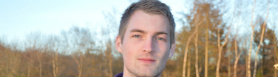
\includegraphics[width=1\textwidth]{img/kent.jpg}
\end{figure}
\section{Introduction}\label{sec:intro}
Intro stuff
\section{Introduction}\label{sec:intro}

%\subsection{Online Video Games}\label{sec:onlinevideogames}

%\emph{League of Legends} (LoL) is an online multiplayer game created by \emph{Riot Games} (Riot). In 2015 LoL was the most played game in the world, with more then 27 million daily players~\cite{LoL27mill}~\cite{LoLmostplayed} .Each player is considered a \emph{summoner}, who has access to \emph{masteries} and \emph{runes} which are selectable additions, used to improve the user controlled \emph{champions}. In a classic 5 versus 5 match, 10 players are divided into the two competing teams; blue and purple. Each player will pick a champion, from a pool of 124 unique champions. Each champion has 5 unique abilities; four actives and one passive. Out of the four actives, one is an ultimate that is extra powerful. Passive abilities cannot be activated by the player. which means it is always active. An \emph{ability} is a magic spell, which does wildly different things, e.g. frost shots that deal damage and slow units, or heals that replenishes health points on target units.

\emph{League of Legends} (LoL) is a PC game created by \emph{Riot Games} (Riot). In the beginning of 2014 LoL had 27 million daily players~\cite{LoL27mill}. One year later it was the most played multiplayer game in the world~\cite{LoLmostplayed}. 
%The game clearly gathers a lot of attention, but not much research in the area of computer science has been published about the game. 
In the following we are going to explain the game, and try ti identify a problem which will be the focus of this project. 

In a classic 5 versus 5 match, 10 players are divided into two competing teams consisting of 5 players each, with the colours blue and purple. Each player is considered a \emph{summoner}, who has access to \emph{masteries} and \emph{runes} which improves the \emph{champions}. They will pick a champion, from a pool of 124 different ones, to use as their playable character. Each champion has 5 unique abilities of which three are active, one is an ultimate that is extra powerful, and one passive, which means it is always active. An \emph{ability} is a magic spell, which does wildly different things, e.g.\ fires a Frost Shot at an opponents champion. 

In \Cref{fig:lolmap} the map is presented, it consists of three lanes identified as \emph{top}, \emph{middle}, and \emph{bottom} which connects the two bases. The blue and purple colours represent the blue and purple teams' respective structures. Circles are \emph{turrets}, pentagons are \emph{inhibitors}, and squares are each team's \emph{nexus}. The green circle indicates \emph{the dragon} and the pink is \emph{the baron}.

\begin{description}
\item[Nexus:] This building spawn \emph{creeps}, which are small monsters with low damage and health, that walks along each of the lanes toward the opposing teams base. Killing these creeps award \emph{gold} and \emph{experience}. When the nexus is destroyed the game ends, making the destroying team the winners
\item[Inhibitor:] When this is destroyed, the destroying teams' minions become stronger on the lane where the inhibitor was placed
\item[Turret:] This is a defensive structure, which fires at nearby enemies
\item[Jungle:] The area between the lanes which hosts stronger
\end{description}

\begin{figure}[!htb]
  \centering
    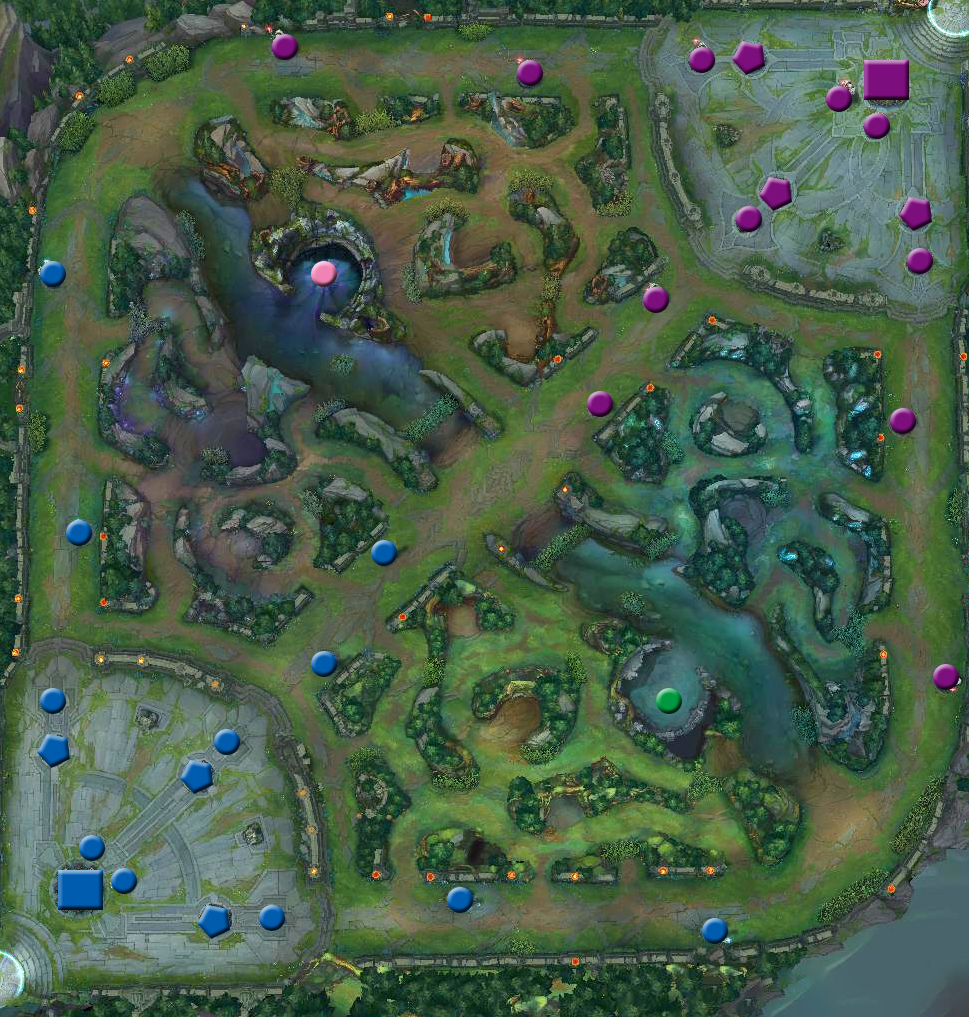
\includegraphics[width=0.6\textwidth]{img/lolmap.jpg}
  \caption{League of Legends map~\cite{lolmap}}\label{fig:lolmap}
\end{figure}

\emph{Creeps} are computer controlled units that are spawned by the nexus and walk toward the opposing teams base. Creeps are spawned by both teams at the same time, which means they will meet at the middle of the lanes, where the majority of the fighting will take place. The dragon is a special stationary and very powerful unit that grants a team a permanent attribute bonus. The baron resembles the dragon, however the attribute bonus is not permanent.

Experience and gold are the currencies of the game, which are earned by killing creeps, monsters, or opposing champions. Both are earned individually by each player. Experience is used to improve the abilities of the champion, while gold is spend purchasing items, that will make the champion more powerful. The game is thus an ever-evolving battle of killing the most units, pushing towards the enemies base, and winning team fights. Usually one team will accumulate an advantage by being ahead in gold, experience, or both, making their champions stronger and making it easier to win fights. When one team is ahead, the other team must play more carefully, adjusting abilities, items and utilising their champions correctly to turn the deficit and get back into the game.

\begin{figure}[!htb]
  \centering
    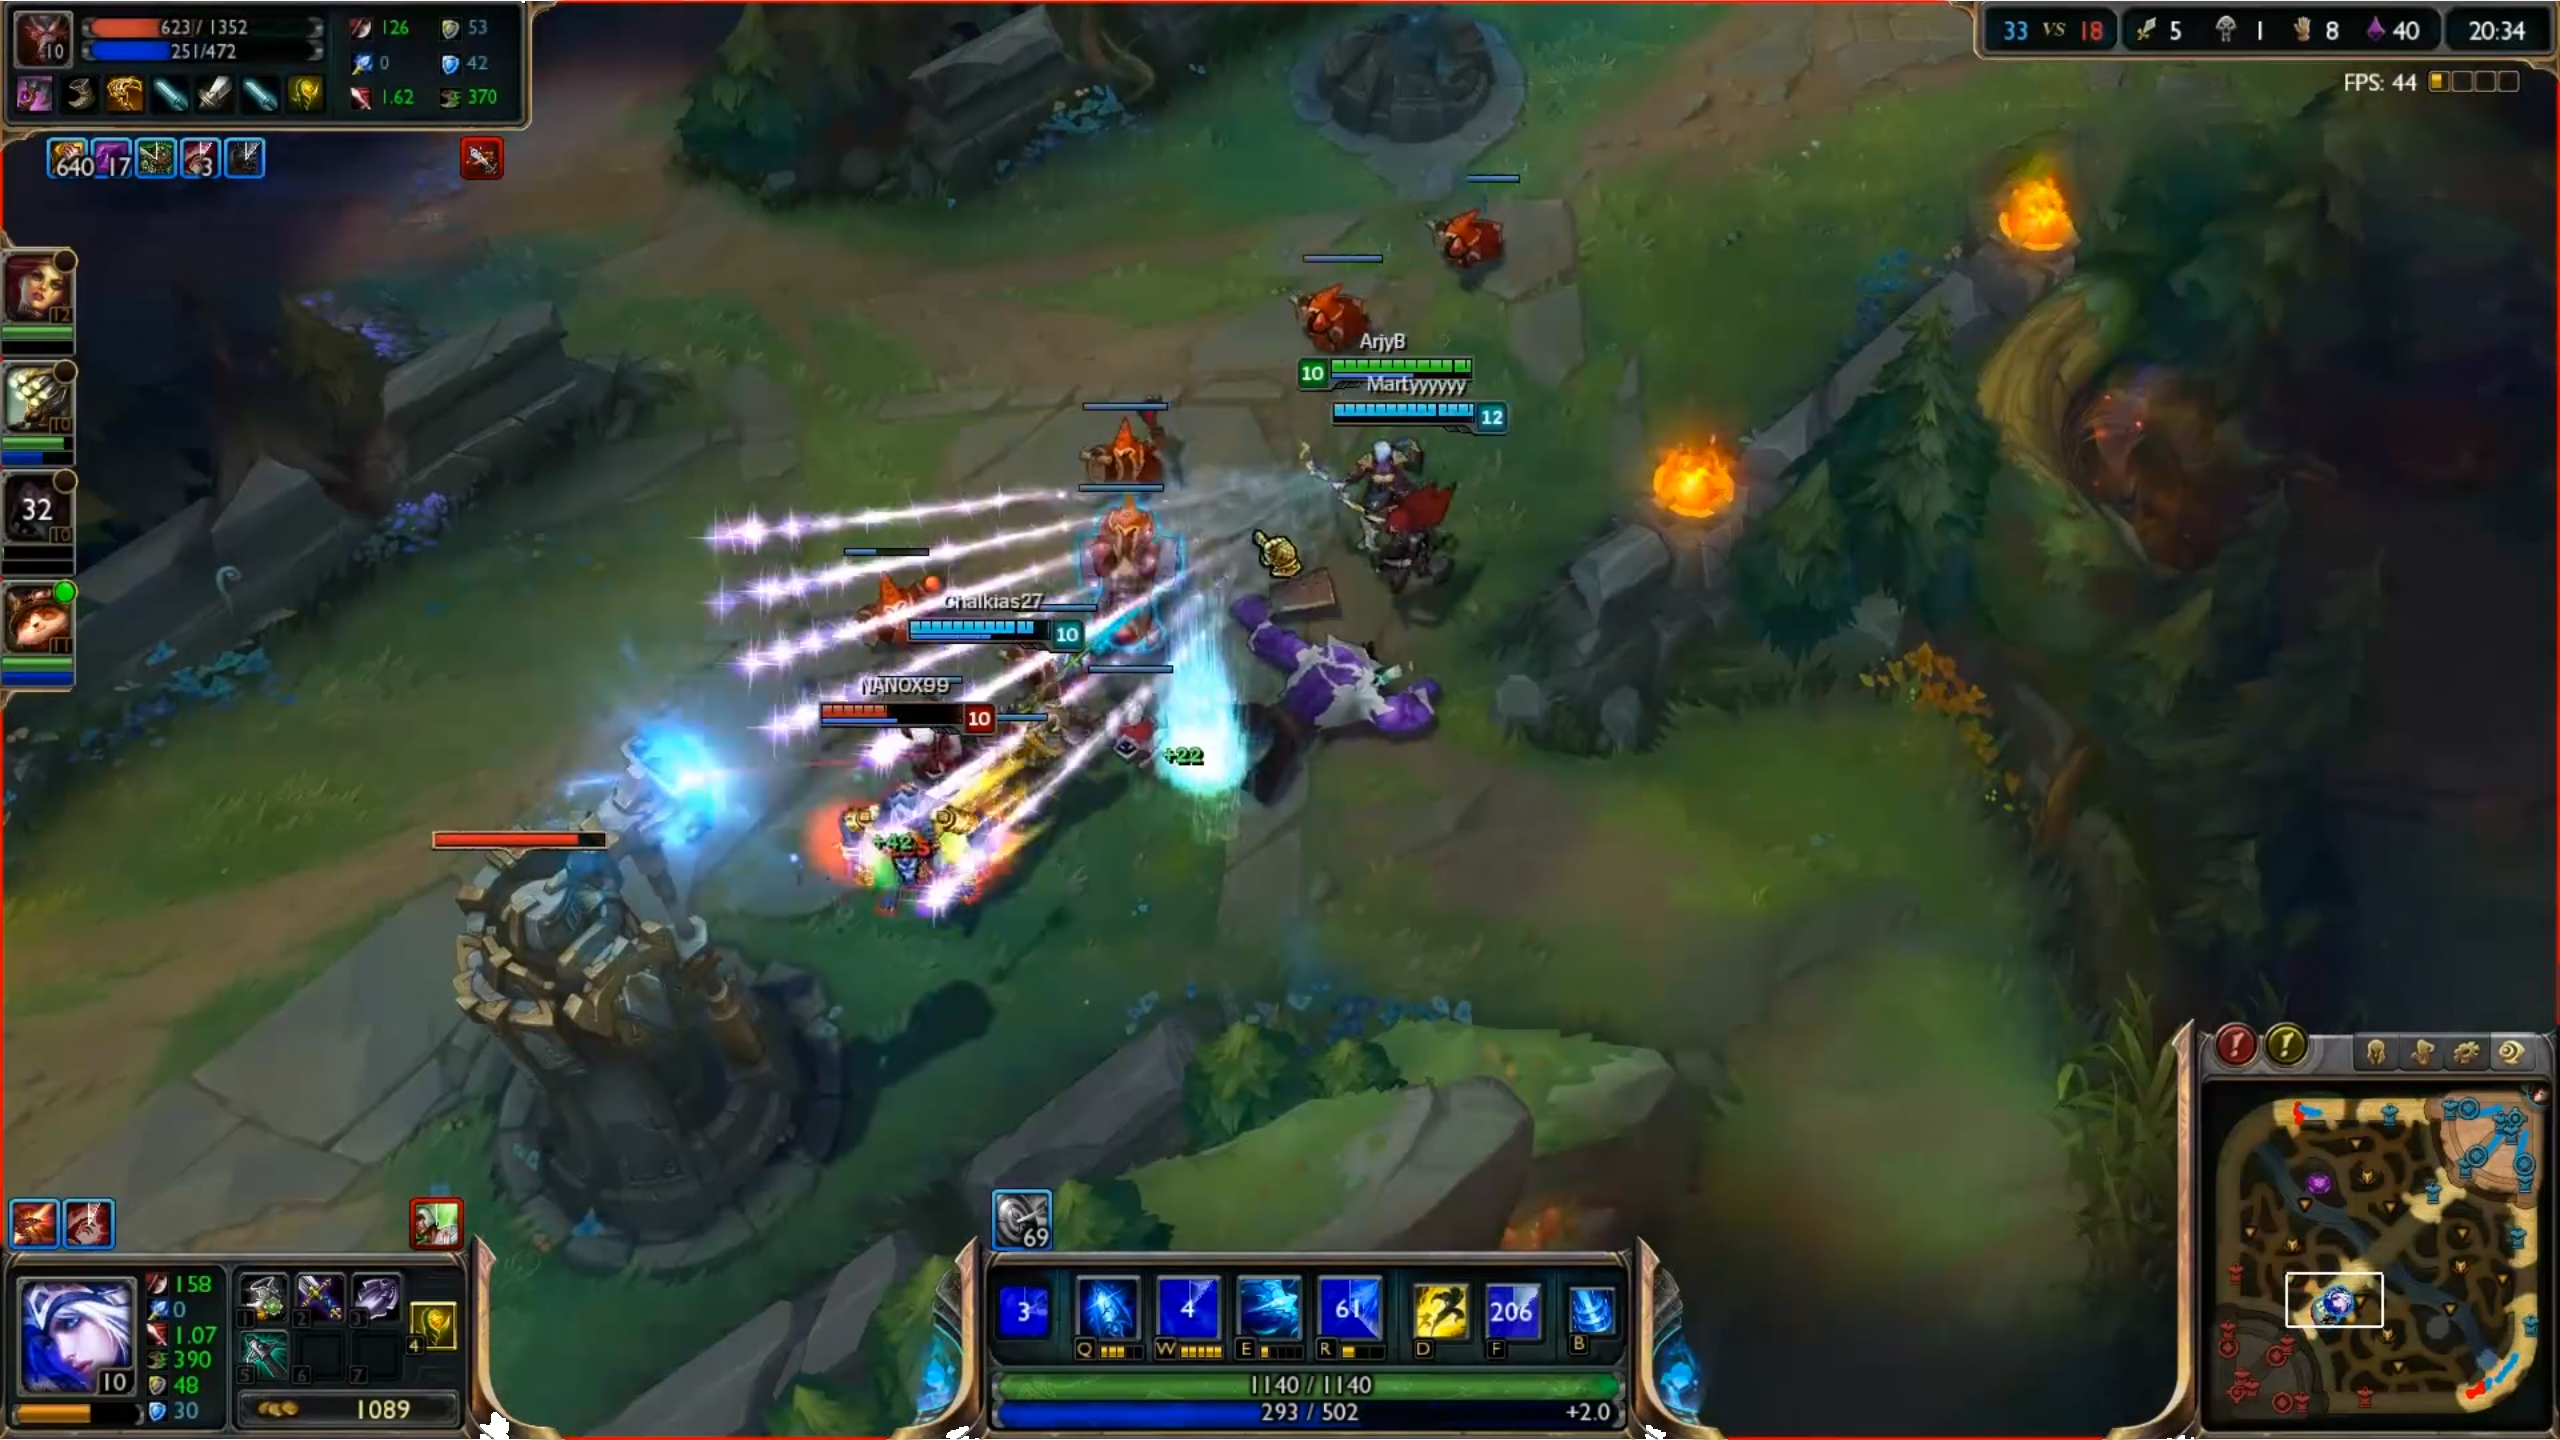
\includegraphics[width=1\textwidth]{img/lolgame.png}
  \caption{Ongoing game: Lower left corner shows the player's chamption equipment and stats. Upper left corner shows a status of friendly champions as well as a summary of a selected champion. Upper right corner shows the current score of the game. The lower right corner shows the map including all structures, friendly units and enemy units in range of friendly units. Lastly in the middle lower screen the champions abilities and health are shown.}\label{fig:lolgame}
\end{figure}

In \Cref{fig:lolgame}, a screenshot of an ongoing game is presented, here the champion \emph{Ashe} uses \emph{Volley} at an enemy player standing near an enemy turret. The description of a subset of Ashe's skills is shown in \Cref{fig:ashe}, including Volley.

\begin{figure}[!htb]
  \centering
  \begin{subfigure}[b]{0.49\textwidth}
    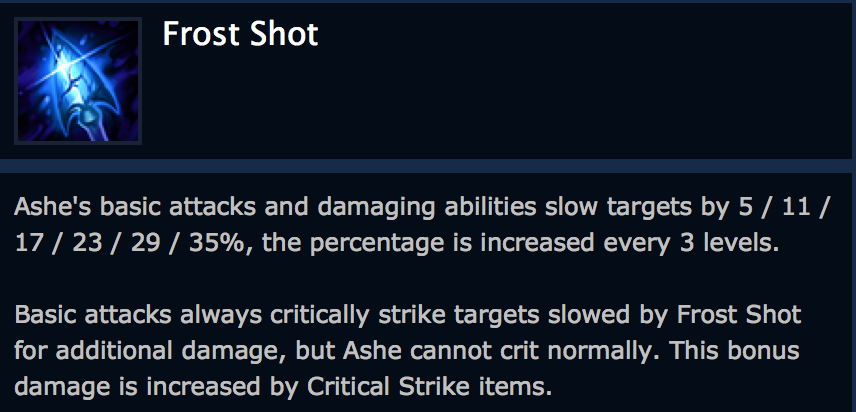
\includegraphics[width=\textwidth]{img/frostshot.png}
    \caption{Example of a passive ability}\label{fig:frostshot}
  \end{subfigure}
  \begin{subfigure}[b]{0.49\textwidth}
    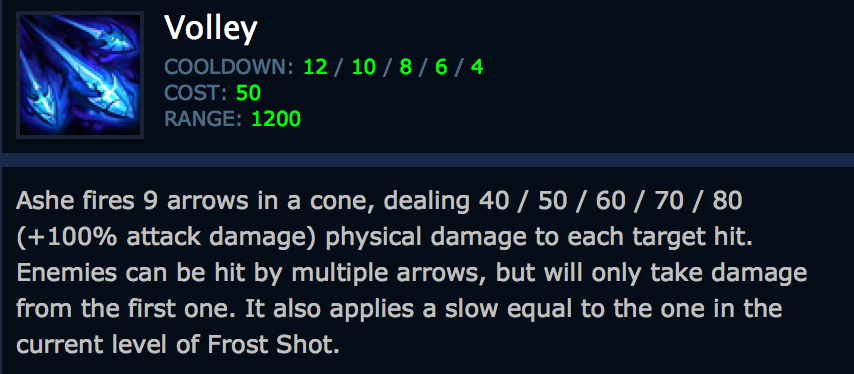
\includegraphics[width=\textwidth]{img/volley.png}
    \caption{Example of an active ability}\label{fig:volley}
  \end{subfigure}
  \begin{subfigure}[b]{0.49\textwidth}
    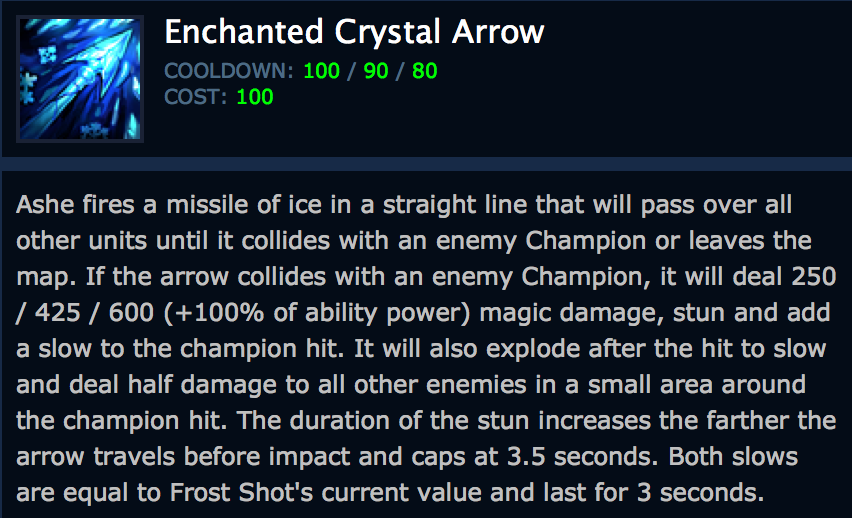
\includegraphics[width=\textwidth]{img/enchanted.png}
    \caption{Example of an ultimate ability}\label{fig:enchanted}
  \end{subfigure}
  \caption{Subset of Ashe's skillset~\cite{ashe}}\label{fig:ashe}
\end{figure}

The game combines strategy, individual player skill, communication, and team play. With a prize pool exceeding \$2,000,000 in the 2014 LoL World Championships, the game attracts serious and highly skilled players~\cite{lolprize}.


%%% Local Variables:
%%% mode: latex
%%% TeX-master: "../main"
%%% End:

\subsection{Machine Learning and Video Games}\label{sec:mlandonlinevideogames}
In video games, one or more players make a number of choices trying to win. The choices made by a single player can be seen as a strategy.
The state space of a video game can be so enormous that it is impossible to comprehend for a human, and hence decisions may be made that are not optimal for winning.
For such video games, machine learning techniques may be able to either outperform human players or provide them valuable support for their decisions.
Machine learning has already been applied to various games, e.g. StarCraft~\cite{Park:2012:PES:2425296.2425298}, Super Mario Bros~\cite{supermario}. and Dota 2~\cite{dota2article}.
Dota 2 is a video game which is very similar to LoL.\@
K.\ Conley and D.\ Perry have trained a classifier to predict the winning team of a Dota 2 match~\cite{dota2article}, by only considering the heroes chosen at the beginning of the game. The classifier can assist players in picking a good combination of heroes.
Each feature used, represents the presence or absence of a particular hero on one of the teams.
When training on 18,000 matches they could correctly predict the outcome of 69.8\% of the 5,669 matches in their test set.
With 50,000 training samples, they almost reached 70\% accuracy. Only matches between players of similar skill levels were considered.

% RELATED WORK ABOUT DISTRIBUTED FILE SYSTEMS AND COMPUTATION
%Konstantin Shvachko, et al.\, created \emph{Hadoop distributed file system} (HDFS), to reliably handle very large data and to stream that data to user application at high %bandwidth. They described the architecture and showed that it can successfully handle 25PB of Yahoo enterprise data~\cite{HDFS}.
%Avinash Lakshman and Prashant Malik created an alternative to Hadoop called Cassandra, which uses Amazon's Dynamo scheme~\cite{ApacheCassandra}.
%Vinod Kumar Vavilapalli et al.\ expanded on Hadoop with YARN, which decoupled the programming model from the resource management infrastructure, it also delegates many of the %scheduling functions to per-application components~\cite{ApacheHadoopYARN}.
%
%Hadoop MapReduce and different variants have successfully been used for big data problems, by distributing the work load between many node in a cluster~\cite{DeanMapReduce}. 
%
%Matei Zaharia, et al.\ have created Apache Spark and using this framework, the computation time is reduced if the data is being reused, in e.g.\ iterative machine learning or 
%iterative data analysis tools~\cite{ApacheSpark}.



%%% Local Variables:
%%% mode: latex
%%% TeX-master: "../main"
%%% End:

\subsection{Motivation}\label{sec:motivation}
As seen in \Cref{sec:mlandonlinevideogames}, a lot of work has been done on machine learning for other video games. LoL is however a rather unexplored game, which is the game this paper will focus on. We wish to help players make strategically good decisions about their champions and summoners. These decisions will analytically be determined by analysing a large quantity of complicated match data. The sheer volume and complexity alone means traditional data processing methods can not effectively be applied, this means we have a \emph{big data problem}. 

A big data problem consists of 3 factors, volume, velocity, and variety. Of the three we have great volume as we have more than 400GB of data, the variety is not an issue as we get all the data from the same source which makes. This ensures that comparing the data input is relatively easy. The final is velocity, we do not take this into consideration as we gather the data one time. If the system should go live, it needs to update as matches are played and patches applied. Then velocity could play a role due to the great number of players and thereby matches being played every day. Every big data problem considers these three variables, but our concern is mainly with volume.

To solve a big data problem, a distributed system of machines must be used, as traditional data processing tools rarely scale well. 

\subsection{Big Data Problem}
A problem can be described as a big data problem if the problem is thoroughly complex, such that conventional data processing cannot be applied. There is no direct definiteion of when something is complex is enough, it is up to the individual solving the problem, if one wishes to apply big data techniques to solve it. However, there are three main variables which contribute to the complexity, namely: Volume, velocity, variety. Volume is the amount of storage the data occupies, velocity is identified as the rate at which the data grows and lastly variety is seen as the complexity or how much variety there is in the data. 
Every problem is thus a combination of these three variables. One might naively think that big data problems are not that different from any other problem, ``just more data!''. The variable which we are concerned with in this project, is mostly the volume. 

In big data problems traditional data processing tools do not scale well. Instead one usually distributes the data across multiple machines using various distributed systems. It is important to recognize that solving a big data problem, introduces new challenges both in terms of storage and complexity. This means that certain machine learning algorithms are more applicable, since the problem will have to be split up and computed in parallel.  We will briefly look at one technique for solving big data problems in the next section.
%http://www.computer.org/csdl/mags/ic/2012/03/mic2012030004.pdf    %From Databases to Big Data

\subsubsection{MapReduce} % (fold)
\label{sec:mapreduce_programming_model}

MapReduce is a programming model which is especially used in the context of ``Big Data''. The model is useful in the context of processing large amounts of data, utilizing parallelization. The main reason for the success of the MapReduce model, is mostly because it is easy for the programmer to parallelize, and its low-cost, high-compute property. MapReduce is well-suited in a distributed computing setting, handling data large enough to not fit into a single disk.

MapReduce is comprised of a \emph{map} procedure and a \emph{reduce} procedure, which is where the name comes from. The two procedures are split into the following actions:


\begin{description}
    \item[Map] This procedure takes as input a key-value pair and ``sets-up'' the data, by e.g.\ filtering or sorting. The resulting output is an intermediate key-value pair used for input to the reduce function.
    \item[Reduce] This procedure takes an intermediate key and a set of values for that key, it then reduces by merging these values into a result
\end{description}
%src: http://static.googleusercontent.com/media/research.google.com/da//archive/mapreduce-osdi04.pdf

\subsubsection{Complications of distributed computing}

Outline of this section:
- Similarity with parallel programming
    - Shared memory vs. network message passing
- Pre-compute feature name/index map
- Transforming/referencing RDD can only happen one at a time
- HDFS data is immutable
- 








%%% Local Variables:
%%% mode: latex
%%% TeX-master: "../main"
%%% End:



\section{Preliminaries}\label{sec:prelim}
In this section, theory or knowledge that is imperative for the understanding of this paper will be presented. In Cref{sec:supervised learning}, several supervised learning concepts will be explained as it is the primary method used in this paper. In \Cref{sec:distributed}, Hadoop filesystem (HDFS) is briefly outlined followed by an introduction to Apache spark which is the cluster computing system mainly used throughout this paper.

\subsection{Logistic Regression}\label{sec:logistic}

To predict the outcome of a match, we use a linear classification model.
The model consists of a hypothesis function that is linear in the parameters.

\[ \hat{y} = w_0 + \sum_{j=1}^{M-1} w_j \phi_j(x) \]

Where $w_j$ represents the impact of of $\phi_j(x)$ on the hypothesis,
$w_0$ is the intercept and $\phi_j$ is a basis function that
performs a transformation on the input features. 

In order to classify the result of the hypothesis function into wins and losses. 
We use the so called logistic or sigmoid function.

\[ \sigma(\textbf{x}) = \frac{1}{1+e^{- \textbf{x}}} \]

The sigmoid function squashes the result of the hypothesis function into an inverval between one and zero.
This is appropriate because we never want a prediction less than zero or greater than one on a binary feature.
Furthermore the sigmoid function has a simple derivative that makes it easy to work with when using iterative methods.

\[ \sigma'(x) = \sigma(x) \times (1-\sigma(x)) \] 

\subsubsection{Cost Function}

In order to find the weights that produce the most accurate classification.
We minimise the squared error function.

\[ E_D = \sum_{n=1}^{N} \left(y_n - \textbf{w} \phi(\textbf{x}_n) \right)^2 \] 

\subsubsection{Regularisation}
To combat the problem of overfitting, we can use a method called L2-Regularisation.
In regularisation we penalise large weights, by adding the following term to the cost function.

\[ E_w = \lambda \sum_{j=1}^{M-1} w_j^2 \]

Where the regularisation constant $\lambda$ scales the penalty. 
The new cost function looks like this.

\[ E(\textbf{w})
  = E_D + E_w 
  = \sum_{n=1}^{N} \left(y_n - \textbf{w} \phi(\textbf{x}_n) \right)^2 + \lambda \sum_{j=1}^{M-1} w_j^2 \]

\begin{flushright}
\cite[online course]{courseraAI}
\end{flushright}

\subsubsection{Batch Gradient Descent}

Since we are using a large number of features, applying an analytic solution to find the weights quickly becomes impractical.
Therefore we use an iterative approach called batch gradient descent.

In gradient descent we iteratively update the weights by the partial derivative of the cost function with respect to the weight, multiplied by a learning rate $\eta$  
\[ w_j \leftarrow w_j - \eta \nabla_w E(\textbf{w}) \]

\subsubsection{Stochastic Gradient Descent}\label{sec:stochastic}

%When dealing with large data sets calculating the sum in the cost function becomes problematic.
 


% Non convergence of stochastic gradient descent





\begin{flushright}
\cite{Bishop2006}[p. ??]
\end{flushright}

% ###################################################################
%
%%\subsection{Logistic Regression}\label{sec:logistic}
%\subsection{Logistic Regression (old)}
%% logistic function
%
%For classification we use an activation function, whose purpose is to squash the result into the interval $(0,1)$.
%\[ f^{\overline{w}}(X_1, X_2, \dots X_n) = f(w_0 + w_1 \times X_1 + w_2 \times X_2 + \cdots + w_n \times X_n) \]
%
%\paragraph{Activation Functions}
%
%The most basic activation function is the so called step function defined as 
%\[ f(x) = \begin{cases}
%%	1 &\text{ if } f^{\overline{w}}(X_1,X_2, \text{ ... }, X_n) > 0 \\
%%	0 &\text{ if } f^{\overline{w}}(X_1,X_2, \text{ ... }, X_n) \leq 0 
%
%	1 &\text{ if } x \geq 0 \\
%	0 &\text{ if } x < 0 
%\end{cases}\]
%
%However the step function is not differentiable, and since this is a requirement for gradient descent we use another
%function called the sigmoid or logistic function.
%\[ f(x) = \frac{1}{1+e^{-x}} \]
%Unlike the previous activation function this function has a very simple derivative.
%
%\[ f'(x) = f(x) \times (1-f(x)) \]
%
%Which makes it easy to implement in a gradient descent algorithm.
%
%The cost function then becomes.
%\[ Error_E(\overline{w}) = \sum_{e \in E} \left(val(e,Y)-f\left(pval^{\overline{w}}(e,Y)\right)\right)^2 \]
%and the partial derivative becomes.
%\[ \frac{\partial \text{Error}_E(\overline{w})}{\partial w_i} 
%	= -2 \times \delta \times f'\left(\sum_i w_i \times val(e,X_i)\right) \times val(e,X_i) \]
%When using the sigmoid activation function the update step in gradient descent looks like this.
%\[ w_i := w_i + \eta \times \delta \times pval^{\overline{w}}(e,Y) \times \left(1 - pval^{\overline{w}}(e,Y)\right) \times val(e,X_i) \]
%
%Where $pval^{\overline{w}}(e,Y) = f(\sum_i w_i \times val(e,X_i))$.  
%
%
%\begin{flushright}
%\cite[p. 306-307]{AI2010}
%\end{flushright}
%
%
%\subsubsection{Regularisation}\label{sec:regular}
%To combat the problem of overfitting, we can use a method called regularisation.
%In regularisation we penalise large weights, by adding the following term to the cost function.
%
%% insert two pictures that show how regularization solves the overfitting problem.
%
%\[ \lambda \sum_{w_i \in \overline{w}} w_i^2 \]
%
%Where the regularisation constant $\lambda$ scales the penalty. 
%The new cost function looks like this.
%
%\[ Error_E(\overline{w}) = \sum_{e \in E} \left(val(e,Y) - pval^{\overline{w}}(e,Y)\right)^2 + \lambda \sum_{w_i \in \overline{w}} w_i^2 \]
%
%
%\begin{flushright}
%\cite[online course]{courseraAI}
%\end{flushright}

%\subsection{Large Datasets}
% Large datasets

% Stochastic regression












%%% Local Variables:
%%% mode: latex
%%% TeX-master: "../main"
%%% End:

\subsection{Computing Distributed Systems}\label{sec:distributed}
In this section we will introduce the distributed systems, which we are going to use. These systems will help us distribute the data across multiple machines, as well as perform distributed parallel computations. 

\subsubsection{Hadoop Distributed Filesystem}\label{sec:hadoopfilesystem}
\emph{Hadoop Distributed Filesystem} (HDFS) is a technology where the main goal is to increase fault tolerance on very large data systems. It is designed to be distributed across inexpensive commodity hardware, where recovery is done quickly and automatically. HDFS operates in a master-worker architecture where the \emph{master} node, maintains the namespace hierarchy as well as the location of file blocks, this machine is called a \emph{namenode}. As shown in \Cref{fig:hadoop}, the namenode can be seen as the root of a HDFS cluster. \emph{Datanodes} take commands from the \emph{namenode}, such as deleting or replicating file blocks.

\begin{figure}[!htb]
  \centering
  \scalebox{0.75}{
    \begin{tikzpicture}[->,>=stealth',bend angle=45,auto]
      % Disks
      \node[cylinder,draw=black,thick,aspect=0.3,minimum height=1.3cm,minimum width=1cm,shape border rotate=90,cylinder uses custom fill,xshift=-5cm] (D1) {Disk};
      \node[cylinder,draw=black,thick,aspect=0.3,minimum height=1.3cm,minimum width=1cm,shape border rotate=90,cylinder uses custom fill,xshift=-2cm] (D2) {Disk};
      \node[cylinder,draw=black,thick,aspect=0.3,minimum height=1.3cm,minimum width=1cm,shape border rotate=90,cylinder uses custom fill,xshift=2cm] (D3) {Disk};
      \node[cylinder,draw=black,thick,aspect=0.3,minimum height=1.3cm,minimum width=1cm,shape border rotate=90,cylinder uses custom fill,xshift=5cm] (D4)  {Disk};
      \node[cylinder,draw=black,thick,aspect=0.3,minimum height=1.3cm,minimum width=1cm,shape border rotate=90,cylinder uses custom fill,xshift=5cm,yshift=5cm] (D5) {Disk};
      \node[cylinder,draw=black,thick,aspect=0.3,minimum height=1.3cm,minimum width=1cm,shape border rotate=90,cylinder uses custom fill,xshift=-5cm,yshift=5cm] (D6) {Disk};

      % Data nodes
      \path node at (0,0) [draw,shape=rectangle, style=rounded corners, minimum width=2cm, minimum height=2.5cm,xshift=-5cm,yshift=0.3cm,label={[yshift=-0.65cm]Data node}] (DN1) {};
      \path node at (0,0) [draw,shape=rectangle, style=rounded corners, minimum width=2cm, minimum height=2.5cm,xshift=-2cm,yshift=0.3cm,label={[yshift=-0.65cm]Data node}] (DN2) {};
      \path node at (0,0) [draw,shape=rectangle, style=rounded corners, minimum width=2cm, minimum height=2.5cm,xshift=2cm,yshift=0.3cm,label={[yshift=-0.65cm]Data node}] (DN3) {};
      \path node at (0,0) [draw,shape=rectangle, style=rounded corners, minimum width=2cm, minimum height=2.5cm,xshift=5cm,yshift=0.3cm,label={[yshift=-0.65cm]Data node}] (DN4) {};
      \path node at (0,0) [draw,shape=rectangle, style=rounded corners, minimum width=2cm, minimum height=2.5cm,xshift=-5cm,yshift=5.3cm,label={[yshift=-0.65cm]Data node}] (DN5) {};
      \path node at (0,0) [draw,shape=rectangle, style=rounded corners, minimum width=2cm, minimum height=2.5cm,xshift=5cm,yshift=5.3cm,label={[yshift=-0.65cm]Data node}] (DN6) {};

      % Namenodes
      \path node at (0,0) [draw,shape=rectangle, style=rounded corners, minimum width=2cm, minimum height=2.5cm,xshift=-2cm,yshift=5.3cm,label={[yshift=-0.65cm]Namenode}] (NN1) {};
      \path node at (0,0) [draw,shape=rectangle, style=rounded corners, minimum width=2cm, minimum height=2.5cm,xshift=2cm,yshift=5.3cm,label={[yshift=-0.65cm]Namenode}] (NN2) {};

      % Server
      \path node at (0,0) [draw,shape=rectangle, style=rounded corners, minimum width=2.5cm, minimum height=3.5cm,xshift=-5cm,yshift=0.6cm,label={[yshift=-0.65cm]Server}] (S1) {};
      \path node at (0,0) [draw,shape=rectangle, style=rounded corners, minimum width=2.5cm, minimum height=3.5cm,xshift=-2cm,yshift=0.6cm,label={[yshift=-0.65cm,xshift=-0.5cm]Server}] (S2) {};
      \path node at (0,0) [draw,shape=rectangle, style=rounded corners, minimum width=2.5cm, minimum height=3.5cm,xshift=5cm,yshift=0.6cm,label={[yshift=-0.65cm]Server}] (S3) {};
      \path node at (0,0) [draw,shape=rectangle, style=rounded corners, minimum width=2.5cm, minimum height=3.5cm,xshift=2cm,yshift=0.6cm,label={[yshift=-0.65cm,xshift=0.5cm]Server}] (S4) {};
      \path node at (0,0) [draw,shape=rectangle, style=rounded corners, minimum width=5.5cm, minimum height=3.5cm,xshift=-3.5cm,yshift=5.6cm,label={[yshift=-0.65cm]Server}] (S5) {};
      \path node at (0,0) [draw,shape=rectangle, style=rounded corners, minimum width=5.5cm, minimum height=3.5cm,xshift=3.5cm,yshift=5.6cm,label={[yshift=-0.65cm]Server}] (S6) {};

      % Cluster
      \path node at (0,0) [draw,shape=rectangle, style=rounded corners, minimum width=6cm, minimum height=9.5cm,xshift=-3.5cm,yshift=3.4cm,label={[yshift=-0.65cm]HDFS Cluster}] (C1) {};
      \path node at (0,0) [draw,shape=rectangle, style=rounded corners, minimum width=6cm, minimum height=9.5cm,xshift=3.5cm,yshift=3.4cm,label={[yshift=-0.65cm]HDFS Cluster}] (C2) {};

      % Stuff
      \path node at (0,0) [draw,shape=rectangle, style=rounded corners, minimum width=1.5cm, minimum height=0.5cm,xshift=-2cm,yshift=9cm,label={[yshift=-0.5cm]Router}] (M1) {};
      \path node at (0,0) [draw,shape=rectangle, style=rounded corners, minimum width=1.5cm, minimum height=0.5cm,xshift=2cm,yshift=9cm,label={[yshift=-0.5cm]Router}] (M2) {};
      \path node at (0,0) [draw,shape=rectangle, style=rounded corners, minimum width=1.5cm, minimum height=0.5cm,xshift=0cm,yshift=10cm,label={[yshift=-0.5cm]Router}] (M3) {};

      % Arrows
      \path (M3) edge (M1)
            (M3) edge (M2)
            (M1) edge (M3)
            (M2) edge (M3)
            (M1) edge (NN1)
            (NN1) edge (M1)
            (M2) edge (NN2)
            (NN2) edge (M2)
            (NN1) edge (DN1)
            (DN1) edge (NN1)
            ([xshift=0.5cm]NN1.south) edge ([xshift=0.5cm]DN2.north)
            ([xshift=0.5cm]DN2.north) edge ([xshift=0.5cm]NN1.south)
            (NN1) edge (DN5)
            (DN5) edge (NN1)
            ([xshift=-0.5cm]NN2.south) edge ([xshift=-0.5cm]DN3.north)
            ([xshift=-0.5cm]DN3.north) edge ([xshift=-0.5cm]NN2.south)
            (NN2) edge (DN4)
            (DN4) edge (NN2)
            (NN2) edge (DN6)
            (DN6) edge (NN2);
          \end{tikzpicture}
      }
      \caption{Hadoop cluster overview}\label{fig:hadoop}
\end{figure} 

Ensuring file coherency in a distributed filesystem can be very complicated, which is why Hadoop employs a simple \emph{write once, read many} model, where new data can either be written as a new file, or appended to an existing file. HDFS is commonly used for file sizes in the giga- and terabyte range. Hadoop \emph{blocks} are used in the same manner as regular blocks on a harddisk, however the size of these block are significantly larger, set to 64MB by default. Larger block size reduce the time spent searching for blocks, relative to the time spent reading them, increasing overall transfer rates of the filesystem. Other central benefits from blocks, are the ability to distribute files larger than any single disk in the cluster, as well as replicate blocks across multiple nodes. 
As default blocks will be replicated to three different locations, where two are placed at the same rack, and the third exist elsewhere in the cluster. The main benefit of block replication is fault tolerance, however the cluster also benefits from better load management and an overall transfer speed increase on files. Fault tolerance of the namenode is also crucial, as the master-worker pattern introduces a single point of failure on the namenode. Hadoop introduces two strategies for handling namenode failure. Firstly, by writing a backup of the filesystems metadata to multiple filesystems. Secondly, by using a secondary namenode, that continuously copy the \emph{edit-log} of the filesystem and periodically merge it with its own filesystem image. However using the secondary namenode alone, presents a risk of loss, as the secondary can lag behind the primary. Commonly both techniques are used, to benefit both from low downtime and no risk of data loss.

To create a file, the HDFS client makes a request on the namenode. If the namenode creates a new file record, the client may then write the file to datanodes. The splitting of data into blocks and placement of blocks on datanodes is managed by a \emph{FSDataOutputStream}, which is a stream given to the HDFS client. The client read files in much the same way as writing them, when a file read is requested, a \emph{FSDataInputStream} is returned to the client. This stream handles which blocks from which locations that should be read. Block replicas are sorted in terms of distance to the client, such that if a block exist on the client itself, this will always be the prioritised block.~\cite{hadoopIntro}.

\subsubsection{MapReduce}\label{sec:mapreduce_programming_model}
MapReduce is a programming model that Hadoop applies. It was developed by J.\@ Dean et al.~\cite{DeanMapReduce}, and is designed to be used in the context of \emph{big data}. The model is useful in the context of processing large amounts of data, clustering as well as utilising parallelism. The main reason for the success of the MapReduce model, is because it is easy for the programmer to do parallel programming, and its low-cost, high-compute property, that supports commodity hardware in a cluster configuration. MapReduce is also well-suited for handling data too large to fit into a single disk.

To program something using MapReduce, one has to write the following two functions. 
\begin{description}\todo{det her er lort og forkert}
\item[Map] works by taking a set of key-value pairs. These pairs are turned into a new set of \emph{intermediate} key-value pairs where the value is now in a list with one element. The intermediate data is now grouped by their key and passed to Reduce.
\item[Reduce] receives the intermediate data, then appends all the values, with the same keys, to a single list with the same key, which is returned as the result.
\end{description}

This can be seen in \Cref{fig:mapreduce}, where the input data of key-value pairs is given to each worker. Each worker then applies the Map function such that $map(k_1,v_1)\rightarrow list\langle k_2,v_2\rangle$, the result is written to disk. The shuffling is then performed: Worker nodes redistribute the data, such that data of some key is placed on the same worker node, effectively grouping by key. Each group can now be reduced by the worker nodes such that $reduce(k_2, list\langle v_2\rangle) \rightarrow list\langle v_3 \rangle$ 

% The user has to construct a \emph{map} and \emph{reduce} procedure. The two procedures are split into the following actions:
%\begin{description}
%\item[Map:] Takes an input key-value pair and produces an \emph{intermediate} set of key-value pairs representing the input. The MapReduce library then groups all the intermediate values by associated keys and pass them to the reduce function.     
%\item[Reduce:] This procedure takes an intermediate key and an iterable set of values for that key, it then reduces by merging these values into a single value result.
%\end{description}

\begin{figure}[!htb]
  \centering
  \scalebox{0.75}{
    \begin{tikzpicture}[->,>=stealth',bend angle=45,auto]
      % Input data
      \path node at (-6,0) [draw,shape=rectangle, style=rounded corners, minimum width=1cm, minimum height=4cm, label={[rotate=90,yshift=-0.35cm,xshift=-2cm]Input Data}] (ID) {};

      % Output data
      \path node at (6,0) [draw,shape=rectangle, style=rounded corners, minimum width=1cm, minimum height=4cm, label={[rotate=90,yshift=-0.35cm,xshift=-2cm]Output Data}] (OD) {};

      % Mappers
      \path node at (-2.5,1.5) [draw,shape=ellipse, style=rounded corners, minimum width=3cm, minimum height=1cm, label={[yshift=-0.8cm]Map}] (M1) {};
      \path node at (-2.5,0) [draw,shape=ellipse, style=rounded corners, minimum width=3cm, minimum height=1cm, label={[yshift=-0.8cm]Map}] (M2) {};
      \path node at (-2.5,-1.5) [draw,shape=ellipse, style=rounded corners, minimum width=3cm, minimum height=1cm, label={[yshift=-0.8cm]Map}] (M3) {};

      % Reducers
      \path node at (2.5,1) [draw,shape=ellipse, style=rounded corners, minimum width=3cm, minimum height=1cm, label={[yshift=-0.75cm]Reduce}] (R1) {};
      \path node at (2.5,-1) [draw,shape=ellipse, style=rounded corners, minimum width=3cm, minimum height=1cm, label={[yshift=-0.75cm]Reduce}] (R2) {};
      
      % Text nodes
      \path node at (-4.75,-2.5) [] (T1) {Split};
      \path node at (-2.5,-2.5) [] (T2) {Map};
      \path node at (0,-2.5) [] (T4) {Shuffle};
      \path node at (2.5,-2.5) [] (T3) {Reduce};
      \path node at (4.75,-2.5) [] (T5) {Merge};

      %Edges
      \path ([yshift=1.465cm]ID.east) edge (M1)
            (ID) edge (M2)
            ([yshift=-1.465cm]ID.east) edge (M3)
            (M1) edge (R1)
            (M1) edge (R2)
            (M2) edge (R1)
            (M2) edge (R2)
            (M3) edge (R1)
            (M3) edge (R2)
            (R1) edge ([yshift=1cm]OD.west)
            (R2) edge ([yshift=-1cm]OD.west);
%       ([xshift=1cm]E2.south) edge ([xshift=1cm]E1.north)
%       (CM) edge (W1)
%       (CM) edge (W2)
%       (W1) edge (CM)
%       (W2) edge (CM)
%       (SC) edge ([yshift=-0.25cm]CM.west)
%       ([yshift=-0.25cm]CM.west) edge (SC)
%       (SC.south east) edge [bend right] (E1.west)
%       (E2.west) edge [bend right] (SC.north east)
%       (SC.north east) edge [bend left] (E2.west)
%       (E1.west) edge [bend left] (SC.south east);

    \end{tikzpicture}
  }
  \caption{The MapReduce programming model}\label{fig:mapreduce}
\end{figure} 

A common MapReduce example is word counting. To use MapReduce for word count on a corpus of documents, each document is passed to a map task which treats each individual word as a key and gives it the value 1. This would give the intermediate result of $\{(w_1,1), (w_2,1),\dots,(w_i,1)\} $. These intermediate results are then grouped by word and distributed across workers assigned to reduce such that all the pairs of e.g.\ $\{w_i,1\}$ are sent to the same worker. Each worker receives a key-value grouping of the form $(w_i, (1,1,\dots) )$. Each worker then sums up the 1's resulting in $(w_i, x)$ where $x>0$. Effectively the output of the reduce task is a list of words and their frequency in the corpus. The pseudocode for word count in MapReduce can be seen in \Cref{lst:mrwordcount}. 
\begin{listing}[H]
\begin{minted}{python}
map(name, document):
  for each word in document:
    emit (word, 1)

reduce(word, partialCounts):
  sum = 0
  for each partialCount in partialCounts:
    sum += partialCount
  emit (word, sum)
\end{minted}
\caption{MapReduce Wordcount}
\label{lst:mrwordcount}
\end{listing}

\subsubsection{Apache Spark}\label{sec:spark}
Apache Spark is a general purpose cluster-computing system, that offers a high level programming API, as well as a set of high level tools for SQL data manipulation, machine learning, and graph processing~\cite{sparkintro}. The main advantage of Spark compared to the MapReduce offered by Hadoop, is when working with iterative processes across the same data. By keeping the data cleverly in memory using Directed Acyclic Graphs, which allows Spark to perform iterative processes faster than Hadoop's MapReduce implementation. An example of an iterative task, is the computation of the gradient for a logistic regression model, where the gradient for the separating hyperplane is found iteratively~\cite{ApacheSpark}.

A Spark application is called a \emph{driver program}. The driver program handles the high level control flow of an application and distributes various operations across the cluster. Spark is comprised of two important abstractions for distributed parallel computation: \emph{resilient distributed datasets} (RDD) and \emph{parallel operations} on these datasets. Furthermore, Spark supports two types of shared variables; broadcast variables and accumulators, that can be used in functions running on the cluster.

The RDD is a read-only collection of objects which is distributed across the machines in the cluster. RDDs are similar to a list structure when working with them. RDDs can live in both memory and on physical structure. They are also fault-tolerant in the sense that they can be rebuilt, because they contain information about how they were built. The parallel operations which are incorporated into Spark are: 
\begin{description}
  \item[Reduce:] Similar to the reduce action in MapReduce 
  \item[Collect:] All elements are sent to the driver program
  \item[Foreach:] Calls a function on each element in the RDD
\end{description}
\Cref{lst:wordcount} shows an example of a Spark application for counting words on a HDFS and output it into standard output.
\begin{listing}[H]
\begin{minted}{python}
  from pyspark import SparkContext
  sc = SparkContext("spark://node1:7077")
  text_file = sc.textFile("hdfs://node1:9000/dictionary.txt")
  counts = text_file.flatMap(lambda line: line.split(" ")) \
                    .map(lambda word: (word, 1)) \
                    .reduceByKey(lambda a, b: a + b)
  print counts.collect()
  \end{minted}
  \caption{Wordcount in Spark on HDFS}
  \label{lst:wordcount}
\end{listing} 
The code can be run by invoking pyspark, which is similar to the python interpreter. When invoked, the application is submitted to Spark on \texttt{spark://node1:7077} through the sparkcontext. \texttt{text\_file} is an RDD with references to each line in the file on the HDFS. We then split each line on blank space, into arrays, which are flattened out by using flatmap. Each word is then sent a key-value pair and reduced by key, counting up the occurrences of the word. Lastly we use collect to print out words and their occurrences.




% \begin{figure}[!htb]
%   \centering
%   \scalebox{0.75}{
%     \begin{tikzpicture}[->,>=stealth',bend angle=45,auto]
%       % Tasks
%       \path node at (0,0) [draw,shape=rectangle, style=rounded corners, minimum width=1.5cm, minimum height=0.8cm,xshift=0cm,yshift=0cm,label={[yshift=-0.65cm]Task}] (T1) {};
%       \path node at (0,0) [draw,shape=rectangle, style=rounded corners, minimum width=1.5cm, minimum height=0.8cm,xshift=2cm,yshift=0cm,label={[yshift=-0.65cm]Task}] (T2) {};
%       \path node at (0,0) [draw,shape=rectangle, style=rounded corners, minimum width=1.5cm, minimum height=0.8cm,xshift=0cm,yshift=4cm,label={[yshift=-0.65cm]Task}] (T3) {};
%       \path node at (0,0) [draw,shape=rectangle, style=rounded corners, minimum width=1.5cm, minimum height=0.8cm,xshift=2cm,yshift=4cm,label={[yshift=-0.65cm]Task}] (T4) {};

%       % Caches
%       \path node at (0,0) [draw,shape=rectangle, style=rounded corners, minimum width=1.5cm, minimum height=0.8cm,xshift=2cm,yshift=1cm,label={[yshift=-0.65cm]Cache}] (C1) {};
%       \path node at (0,0) [draw,shape=rectangle, style=rounded corners, minimum width=1.5cm, minimum height=0.8cm,xshift=2cm,yshift=5cm,label={[yshift=-0.65cm]Cache}] (C2) {};

%       % Executor
%       \path node at (0,0) [draw,shape=rectangle, style=rounded corners, minimum width=3.75cm, minimum height=2.15cm,xshift=1cm,yshift=0.5cm,label={[yshift=-0.85cm,xshift=-1cm]Executor}] (E1) {};
%       \path node at (0,0) [draw,shape=rectangle, style=rounded corners, minimum width=3.75cm, minimum height=2.15cm,xshift=1cm,yshift=4.5cm,label={[yshift=-0.85cm,xshift=-1cm]Executor}] (E2) {};

%       % Worker
%       \path node at (0,0) [draw,shape=rectangle, style=rounded corners, minimum width=3.95cm, minimum height=3cm,xshift=1cm,yshift=0.75cm,label={[yshift=-0.55cm,xshift=-0.8cm]Worker node}] (W1) {};
%       \path node at (0,0) [draw,shape=rectangle, style=rounded corners, minimum width=3.95cm, minimum height=3cm,xshift=1cm,yshift=4.75cm,label={[yshift=-0.55cm,xshift=-0.8cm]Worker node}] (W2) {};

%       % Cluster Manager
%       \path node at (0,0) [draw,shape=rectangle, style=rounded corners, minimum width=3.5cm, minimum height=2cm,xshift=-4cm,yshift=2.75cm,label={[yshift=-1.25cm]Cluster manager}] (CM) {};

%       % SparkContent
%       \path node at (0,0) [draw,shape=rectangle, style=rounded corners, minimum width=3.25cm, minimum height=1cm,xshift=-9cm,yshift=2.5cm,label={[yshift=-0.80cm]SparkContent}] (SC) {};

%       % Driver Program
%       \path node at (0,0) [draw,shape=rectangle, style=rounded corners, minimum width=3.5cm, minimum height=2cm,xshift=-9cm,yshift=2.75cm,label={[yshift=-0.65cm]Driver Program}] (DP) {};

%       % Edges
%       \path ([xshift=1cm]E1.north) edge ([xshift=1cm]E2.south)
%       ([xshift=1cm]E2.south) edge ([xshift=1cm]E1.north)
%       (CM) edge (W1)
%       (CM) edge (W2)
%       (W1) edge (CM)
%       (W2) edge (CM)
%       (SC) edge ([yshift=-0.25cm]CM.west)
%       ([yshift=-0.25cm]CM.west) edge (SC)
%       (SC.south east) edge [bend right] (E1.west)
%       (E2.west) edge [bend right] (SC.north east)
%       (SC.north east) edge [bend left] (E2.west)
%       (E1.west) edge [bend left] (SC.south east);

%     \end{tikzpicture}
%   }
%   \caption{Spark setup overview}\label{fig:spark}
% \end{figure} 

%%% Local Variables:
%%% mode: latex
%%% TeX-master: "../main"
%%% End:


\section{Data and Prediction Setup}\label{sec:features}
In \Cref{sec:matchdata} we investigate the match data made available by the Riot Games API, which covers almost any detail of a given LoL match.
\Cref{sec:choosingfeatures} identifies a number of features that can be extracted from match data, which we think are most important when it comes to prediction of the winning team. The choice is based on our intuition as more or less experience LoL players. The size of each type of feature's domain is calculated in \Cref{sec:featuresparsity}, as well as the sparsity with regards how many features that appear in each match.
In \Cref{sec:representationoffeatures}, a possible feature symmetry is investigated which raises a number of concerns as to how the extracted features should be represented. 
\section{Data and Feature Setup}\label{sec:features}
In \Cref{sec:matchdata} we investigate the match data made available by the Riot's API, which covers almost any detail of a match.
\Cref{sec:choosingfeatures} identifies a number of features that can be extracted from match data, which we think are most important when it comes to prediction of the winning team. The choice is based on our intuition as more or less experienced LoL players. The size of each type of features domain is calculated in \Cref{sec:featuresparsity}, as well as the sparsity with regards to how many features that appear in each match.
In \Cref{sec:representationoffeatures}, a possible feature symmetry issue is investigated which raises a number of concerns and suggestions for solutions as to how the extracted features should be represented. 


\subsection{League of Legends Match Information}\label{sec:matchdata}
Riot records large amounts of information about played matches and players~\cite{matchinfo}. Much, if not all, of this data is publicly available through their online API. In this paper the focus will be on the match data only, and more particularly the data that can be extracted before a match starts. The only exception is information about which team that won each match. Since we want to predict who wins, we need that data to train and evaluate a classifier.
We have chosen to extract the following data from each match:
\begin{itemize}
\item Winning team
\item Champions on each of the two teams
\item The rank of all players
\item Game mode
\item Queue type
\end{itemize}
And the following data from each player:
\begin{itemize}
\item Lane occupied 
\item Runes 
\item Masteries 
\item Summoner spells 
\end{itemize}
All the extracted information has be chosen because we think it might be useful for estimating how good a particular team is against another team. \todo{kommetar: dårlig begrundelse}
The champions on each of the two teams have been included because some champions may be better than others.
The rank of players are considered because the rank system in LoL aims to assign better players a greater rank. Intuitively, a team of high ranked players must be better than a team of low ranked players.
The lane played by each player may be useful, because players often stick to one particular lane for the first half a match.
Note that the lanes of the opponent team is not known before the game starts, but we have still chosen to include it, because it very often can determined based on the picked champions. Knowing the lane of the players means knowing the ranks and champion of the players that most often fights against each other.
Both the masteries, runes. and summoner spells are worth knowing, because each of them add or improve some property of a champion. 
%The summoner spells are also worth considering because they adds additional properties to a champion.
Different game modes imply different play styles. By only considering the 5 versus 5 game mode, we hope to achieve better predictions.
The queue type of the match lets us know if the LoL match making system has formed the two teams, or the players have formed the two teams themselves.
Teams formed on their own may be better, because the players in self formed teams often know each other better and more often use voice communication tools.
Finally the matches patch version is used to make sure that we only use matches from the same patches. Different patches may change aspects of the game, e.g.\ the strength of particular champions, and without accounting for different patches, the trained classifier accuracy may decrease.  

The data set we use use consists of matches played from $23^{\text{rd}}$ of March 2015 to $27^{\text{th}}$ of March 2015. It includes match details for matches played across the world. When filtering the games to include only 5 versus 5 game modes, we are left with 1925980 matches. The patch version of all matches used is $5.6$.


%%% Local Variables:
%%% mode: latex
%%% TeX-master: "../main"
%%% End:

\subsection{Choosing features}\label{sec:choosingfeatures}
In the following, we aim to define the features $\phi_j(x)$ for each LoL match $x$, as described in \Cref{sec:phi}.
We define 5 different types of features and argue argue why each type is a good candidates for predicting the winning team.
The different types of features are each extracted by a mapping function, that maps a LoL match (in some cases with additional parameters) to a value. 
Before the feature mappings are defined, convenient notations are introduced that mathematically describes the concept of a game.
$C = \{1, 2, \dots, m\}$ is the set of all champions, where each champion is represented by an id. $m = 124$ for the patch version of LoL used in this project.
$P = \{p_1, p_2, \dots\}$ denotes the set of all players.
$T(x) = \{T_\text{blue}$, $T_\text{purple}\}$ is a set containing the two teams of match $x$, namely \emph{blue} and \emph{purple} respectively.
$T_i(x) = \{ (p_j, c_j) \in P \times C \mid c_j \text{ is controlled by } p_j \text{ on team } i  \text{ in match } x \}$.
$R = \{\text{unranked},\text{bronze},\text{silver},\text{gold},\text{platinum},\text{diamond},\text{master},\text{challenger},\}$ is the set of ranks.
$L = \{\text{top},\text{bottom},\text{mid},\text{jungle},\}$ is the set of lanes.
Some champions may be better than other champions. To capture the strength of individual champions, we will need a feature that represent the presence or absence of a particular champion on each team.
We define a feature $\phi_{\text{SINGLE}, t, c}(x)$, such that $\forall t \in T(x), \forall c \in C:$
\begin{equation}\label{eq:single}  
\phi_{\text{SINGLE}, t, c}(x) = 
\begin{cases} 
  1 & \text{if } (c, p) \in t \text{ for some } p \\
  0 & \text{otherwise} 
\end{cases}
\end{equation}



Some champions are considered damage dealers, they deal very high damage, but die easily. Other champions deal very little damage, but can be almost impossible to kill, these are considered tanks. These two types of champions are weak when alone, but when they team up, they can pose a serious threat. The tank can be used by the damage dealer as a living shield, allowing him to stay alive for much longer, thus deal more damage.
To capture the synergy between two champions on the same team, we will for each team need a feature that represents the presence or absence of every 2-combination of champions on that team. Therefore, we define a feature $\phi_{\text{PAIR},t, c_1, c_2}(x)$ such that $\forall t \in T(x), \forall c_1, c_2 \in C$ where $c_1 < c_2$:
\begin{equation}\label{eq:pair}
\phi_{\text{PAIR}, t, c_1, c_2}(x) =
\begin{cases}
  1 & \text{if } (c_1, p_1), (c_2, p_2) \in t \text{ for some }p_1, p_2\\
  0 & \text{otherwise}
\end{cases}
\end{equation}

We make the restriction $c_1 < c_2$, because we want to ignore permutations. This is because the two features $x_\text{PAIR}(t, c_1, c_2)$ and $x_\text{PAIR}(t, c_2, c_1)$ are the same, since they both capture that the two champions $c_1$ and $c_2$ are present on team $t$.

Some champions may have an advantage when fighting against a particular opponent.
For instance, a champion that is good at dodging ranged attacks is good against an enemy that only has ranged attacks.
We say that the better suited champion \emph{counters} the other.
To capture that one champion may counter another, we will for each champion on team $t$ need a feature that represents the presence or absence of every possible champion on the other team.
We define a feature $\phi_{\text{COUNTER},c_1,c_2}(x)$ such that $\forall c_1, c_2 \in C:$
\begin{equation}\label{eq:counter}
\phi_{\text{COUNTER},c_1,c_2}(x) = 
\begin{cases} 
1 & \text{if } (c_1, p_1) \in T_\text{blue}(x) \text{ and } (c_2, p_2) \in T_\text{purple}(x) \text{ for some } p_1, p_2 \\ 
0 & \text{otherwise} 
\end{cases}
\end{equation}

In this case, we do not have the restriction $c_1 < c_2$ and thus consider permutations instead of combinations.
To understand why, consider that $c_1$ counters $c_2$.
In this case, the feature $\phi_{\text{COUNTER},c_1,c_2}(x) = 1$ is favorable to the blue team, while $\phi_{\text{COUNTER},c_2,c_1}(x) = 1$ is favorable to the red team.
Note that in some game modes, $\phi_{\text{COUNTER},c_1,c_2}(x) = 1$, is allowed for $c_1 = c_2$. That is, the same champion may appear on both teams.
In that way we can capture if a champion can counter itself due to some asymmetries in the map layout.

In LoL, players can compete in ranked games, where they are placed in one of 7 tiers. Better players achieve higher tiers.
Before a match starts, we have access to data about the highest tier each player has achieved in a ranked game, which we will refer to as the rank of a player. We also know if a player has not competed in ranked games, in which case we say that he is unranked.
A player can achieve one of the ranks \textit{bronze}, \textit{silver}, \textit{gold}, \textit{platinum}, \textit{diamond}, \textit{master}, \textit{challenger} (mentioned in increasing order of skills required to achieve the rank).
We define a score function $\varphi : P \rightarrow \mathcal{N}$, where $\varphi(p) = 0$ if $p$ is unranked, or $1, 2, \dots, 7$ if $p$ has rank \textit{bronze}, \textit{silver}, $\dots$, \textit{challenger} respectively.
We define the rank of a team to be the average rank of all players on that team who is not unranked:
\begin{equation}\label{eq:eta}
\eta(t) = \frac{\sum\limits_{(p, c) \in t} \varphi(p)}{|\{(p, c) \in t \mid \varphi(p) > 0\}|}
\end{equation}
which we use to define a single feature
\begin{equation}\label{eq:bestrank}
\phi_\text{BEST-RANK}(x) = 
\begin{cases} 
  1 & \text{if } \eta(T_\text{blue}(x)) > \eta(T_\text{purple}(x))\\
  -1 & \text{if } \eta(T_\text{blue}(x)) < \eta(T_\text{blue}(x))\\
  0 & \text{otherwise} 
\end{cases}  
\end{equation}

The $\phi_\text{BEST-RANK}$ feature may have some shortcomings. The assumption that the rank of each player can be mapped to a score on a linear scale may not be entirely on spot.
Also, it may be easier to predict one team to be a winner, if the average rank of the two teams are considerably different. That is, if the players on one of the team have much greater ranks in average. The difference between the average rank of each team is not captured by the $\phi_\text{BEST-RANK}$ feature.
Therefore, another type of feature $\phi_{\text{PLAYER-RANK},p}(x)$ is introduced that captures the exact rank of each player.
$\forall(p, c) \in T_\text{blue}(x) \cup T_\text{purple}(x)$, we define a feature
\begin{equation}\label{eq:playerrank}
\phi_{\text{PLAYER-RANK},p}(x) = S(p)  
\end{equation}

In the early stage of a match, players tend to keep their champion in the same lane.
If a good player plays against a bad player in the same lane, the good player might get so strong, that the good player is able to carry the team to victory.
To define a new feature that considers the rank of players that play against each other in the same lane,
we first define a function that given a lane and team returns the rank of all players on the team that plays in that lane.
$\forall l \in L, \forall t \in T(x)$, we define
\begin{equation}\label{eq:xi}
  \xi(t,l) =
\begin{cases} 
  \text{none} & \text{if } \forall(c, p) \in t: c \text{ does not play in lane } l. \\
  r_1 & \text{if only } (c_1, p_1) \in t \text{ plays lane } l \text{ and } p_1 \text{ has rank } r_1 \text{.}\\
  (r_1, r_2) & \text{if only } (c_1, p_1), (c_2, p_2) \in t \text{ plays lane } l, \text{ where } p_1, p_2 \text{ has rank } r_1, r_2\\ 
&\text{respectively, and } p_1 \neq p_2.\\
  \text{many} & \text{otherwise}.
\end{cases}
\end{equation}

$\forall l \in L$, and for any $a,b$ that are possibles values in the range of $\xi$, we define the feature
\begin{equation}\label{eq:laneranks}
\phi_{\text{LANE-RANKS},l,a,b}(x) =
\begin{cases} 
  1 & \text{if } \xi(T_\text{BLUE}(x),l) = a, \xi(T_\text{PURPLE}(x),l) = b\\
  0 & \text{otherwise} 
\end{cases}  
\end{equation}

Some champions are better suited for a particular lane. For instance, mages tend to go mid as they generally loose both mana and health fast, and the path back to the base for regeneration is shortest from mid.
$\forall l \in L, \forall(p, c) \in T_\text{blue}(x) \cup T_\text{purple}(x)$, we define a feature
\begin{equation}\label{eq:championlane}
  \phi_{\text{CHAMPION-LANE},c,l}(x) =
\begin{cases} 
  1 & \text{if champion } c \text{ fought at lane } l)\\
  0 & \text{otherwise} 
\end{cases}
\end{equation}

\subsection{Feature sparsity}\label{sec:featuresparsity}
The size of $\phi_{\text{SINGLE}}$ is $|T(x)| \cdot |C| = 2 \cdot 124 = 248$. In each match, only $2 \cdot 5 = 10$ of those features appear. By appearance, we mean having a value of 1.\\
The size of $\phi_{\text{PAIR}}$ is $|T(x)| \cdot |C| \cdot (|C|-1) / 2 = 2 \cdot 124 \cdot 123 / 2 = 15252$. In each match, only $2 \cdot 5 \cdot 4 / 2 = 20$ of those features appear.\\
The size of $\phi_{\text{COUNTER}}$ is $|C|^2 = 124^2 = 15376$. In each match, only $5 \cdot 5 = 25$ of those features appear.\\
The size of $\phi_{\text{BEST-RANK}}$ is 3 by definition. In each match, only $1$ of those features appear.\\
The size of $\phi_{\text{PLAYER-RANK}}$ is $2 \cdot 5 \cdot 8 = 80$, since each of the $2$ teams have $5$ players, that each can have $1$ of $8$ ranks. In each match, only $10$ features appear, because each player has only $1$ rank.\\
The size of $\phi_{\text{LANE-RANKS}}$ is $|L| \cdot (2 + |R| + |R|^2)^2 = 21904$, because each lane contains either none, 1, 2, or many champions from each team.
In each match only $5$ of these features appear, as each of the lanes has exactly one combination of ranks of the players / champions playing against each other.
The size of $\phi_{\text{CHAMPION-LANE}}$ is $|T(x)| \cdot |C| \cdot |L| = 2 \cdot 124 \cdot 4 = 992$, because for each team, every champion can be in one of the 4 lanes. In each match, only $2 \cdot 5 \cdot 4 = 40$ features appear. 
These figures are presented in \Cref{tab:featuresparsity}, which also includes the number of features that appeared in $60.000$ LoL matches.

\begin{center}
\begin{table}[h]
\begin{tabular}{|l|ccc|}
\hline
Feature type                & Domain size & Appears in a single match & Appeared in 60,000 matches \\ \hline
$\phi_{\text{SINGLE}}$      & 248         & 10 & 248               \\ 
$\phi_{\text{PAIR}}$        & 15252       & 20 &                   \\ 
$\phi_{\text{COUNTER}}$     & 15376       & 25 & 15359             \\ 
$\phi_{\text{BEST-RANK}}$   & 3           & 1  & 3                 \\ 
$\phi_{\text{PLAYER-RANK}}$ & 80          & 10 & 80                \\ 
$\phi_{\text{LANE-RANKS}}$  & 21904       & 5  & 1834              \\ 
$\phi_{\text{CHAMPION-LANE}}$ & 992       & 40 & 992               \\ \hline
\end{tabular}
\caption{The sparsity of each type of feature}\label{tab:featuresparsity}
\end{table}
\end{center}

%%% Local Variables:
%%% mode: latex
%%% TeX-master: "../main"
%%% End:


\section{Representation of features}
\label{sec:representationoffeatures}
From the definition of features in section \ref{sec:choosingfeatures}, we can calculate that

\[|X_1| = |T| \cdot m \]

\[|X_2| = |T| \cdot \frac{m(m-1)}{2} \]

\[|X_3| = m^2  \]

where $m = |C|$ is the total number of champions in LoL.

With 123 total champions in LoL, we have that for each match:
$2 \cdot 5 = 10$ $X_1$ features are present out of 246 possible.
$2 \cdot (5 \cdot 4)/2 = 20$ $X_2$ features are present out of 15006 possible.
$5 \cdot 5 = 25$ $X_3$ features are present out of 15129 possible.
By present, we mean the features which value is 1.
It is clear that only a sparse number of features are present in each game. 

For optimizing the machine learning methods used, we will for each match only represent the features that are present in that game. 
Before applying a machine learning method, each of the features introduced in section \ref{sec:choosingfeatures} are assigned a unique ID.
For each match in the training data, the machine learning method is then given the IDs of the features present in that match.
We will now show how each feature in $X_1$, $X_2$, and $X_3$ is assigned a unique id:

\begin{center}
Every feature $x_1(t, c) \in X_1$ is given the ID:
\[ c + t \frac{|X_1|}{|T|} \]
\end{center}

It is easy to see that this assign unique IDs to all features in $X_1$.
Assigning unique IDs to features in $X_2$ is a bit more tricky since we are dealing with combinations and thus have the restriction $c_1 < c_2$.
If we enumerate all features $x_2(t, c_1, c_2) \in X_2$ for a single $t$ by $(c_1, c_2)$, we get the following enumeration:
\begin{align*}
(0, 1), (0, 2), (0, 3),& \dots, (0, m-1)\\
        (1, 2), (1, 3),& \dots, (1, m-1)\\
                        & \vdots    \\
                         &      (m-2, m-1)\\                   
\end{align*}
If using row and column indexes starting at $0$, we see that row $0$ contains $m-1$ elements, row $1$ contains $m-2$ elements, and so on.
That is, any row $i$ contains $m-1-i$ elements.
It is clear that the combination $(c_1, c_2)$ lies in row $c_1$ as element $c_2 - 1 - c_1$.
Thus, any combination $(c_1, c_2)$ is preceded by all elements in row $0$ through $c_1 - 1$, as well as $c_2 - 1 - c_1$ elements in its own row.
The number of elements in row $0$ through $c_1 - 1$ is an arithmetic series, and we can calculate the total number of elements
using the formula $n(a_0 + a_{n-1}/2$, where $n$ is the number of rows and $a_i$ is the number of elements in row $i$.
Since we have $m-1$ elements in row $0$ and $m - 1 - (c_1 - 1)$ elements in row $c_1 - 1$,
we get that $c_1(m-1 + m-1-(c_1-1))/2 = c_1(2m-1-c_1)/2$ elements are contained in the rows $0$ through $c_1 - 1$.
By adding the number of elements preceding $(c_1, c_2)$ in its own row, we get that $(c_1, c_2)$ is preceded by a total of
$c_1(2m-1-c_1)/2 + c_2-1-c_1 = c_1(2m-3-c_1)/2 + c_2-1$ elements.
We can now use the number of elements that precede $(c_1, c_2)$ as the ID for the feature $x_3(t, c_1, c_2)$. However, we must remember to add the offset $2m$, to not clash with the $x_t(c)$ features, and we must also add the offset $t \cdot m(m-1)/2$ since we for each $t \in T$ have $m(m-1)/2$ of the $x_3(t, c_1, c_2)$ features.
We finally get that:

\begin{center}
Every feature $x_2(t, c_1, c_2) \in X_2$, is given the ID:
\[ |X_1| + t \cdot \frac{|X_2|}{|T|} + \frac{c_1(2m-3-c_1)}{2} + c_2-1\]
\end{center}

Assigning an ID to the features in $X_3$ is simple since we are dealing with permutations. If we start enumerating all those features in the same way we did for the $X_2$ features, we will quickly see that the feature $x_3(c_1, c_2)$ appears as the $c_1m+c_2$'th element in the enumeration.
Now, we only need to add the correct offset of $|X_1| + |X_2| + |X_3|$, to get that:
\begin{center}
Every feature $x_3(c_1, c_2) \in X_4$ is given the ID:
\[|X_1| + |X_2| + c_1m+c_2\]
\end{center}

%%% Local Variables:
%%% mode: latex
%%% TeX-master: "../main"
%%% End:

\section{Cluster}\label{sec:cluster}
In this section the cluster that will be doing the computations will be outlined. In \Cref{sec:clustersetup} the setup of the cluster and the available resources are listed, followed by a profile of the resource usage in \Cref{sec:profile}.
\section{Cluster}\label{sec:cluster}
In this section, the cluster that will be doing the computations will be outlined. In \Cref{sec:clustersetup} the setup of the cluster and the available resources are listed, followed by a profile of the resource usage in \Cref{sec:profile}. In \Cref{sec:speedup} the speedup from using additional nodes for computations will be measured, both using several nodes and computation speed.

\subsection{Cluster Setup}\label{sec:clustersetup}

The cluster used for this work consist of four nodes, one master and three worker nodes. The master is master both in terms of cluster management on Spark and storage management on HDFS.\ Because of the limited resources for the project and small size of the cluster and dataset, some of the common fault tolerance functionality of Hadoop and Spark has not been employed. Most significantly, only one replication of data exist across HDFS, which naturally put large parts of the data at risk, however given the relatively small amount of machines and ease of access to new match data, we chose to prioritise data volume over fault tolerance. There are two unique setups of the nodes which can be seen in \Cref{tab:setups}.
\begin{table}[!htb]
  \centering
  \begin{tabular}{|r|ccc|}
    \hline
      & CPU & Storage & Memory \\\hline
    Setup 1 & Dual core intel e8400 3Ghz & 220 GB 7200 RPM & 4GB DDR2 \\
    Setup 2 & Quad core intel q9400 2.66Ghz & 220 GB 7200 RPM & 8GB DDR2 \\\hline
  \end{tabular}
  \caption{The different node setups}\label{tab:setups}
\end{table}

Where the master and one worker node has a dual core and the two remaining worker nodes have the quad cores. The machines are linked together using a switch capable of 200Mbit pr port, which sets a potential one-way bandwidth of 12.5MB/s pr machine. The physical setup of the cluster can be seen in \Cref{fig:clustersetup}.

\begin{figure}[!htb]
  \centering
    \includegraphics[width=1\textwidth]{img/cluster2.jpg}
  \caption{Physical cluster setup}\label{fig:clustersetup}
\end{figure}

%%% Local Variables:
%%% mode: latex
%%% TeX-master: "../main"
%%% End:

\subsection{Hadoop Filesystem}\label{sec:hadoopfilesystem}

Hadoop filesystem (HDFS) is a distributed filesystem that seeks to increase fault tolerance on very large datasystems. The filesystem is designed to be distributed across inexpensive commodity hardware, where recovery is done quickly and automatically. HDFS is run on a cluster, where one machine exist as a \emph{name node}, which is a central node that manages the location of file blocks. Blocks are used as a means to split large files, replicate and distribute them across the cluster’s \emph{data nodes}. Ensuring file coherency could become very complicated in such a system, which is why Hadoop implements a simple “write once, read many” model. It is common that the files used with Hadoop is of the Gigabyte-Terabyte size.
As seen in \Cref{fig:hadoop}, the name node can be seen as the root of a HDFS cluster. An application access data by first requesting the locations of a file’s blocks from the name node and then use those locations to read directly from data nodes. As described earlier the cluster used for this project, consists of the central name node and three data nodes~\cite{hadoopIntro}. 

\begin{figure}[!htb]
  \centering
  \scalebox{0.75}{
    \begin{tikzpicture}[->,>=stealth',bend angle=45,auto]
      % Disks
      \node[cylinder,draw=black,thick,aspect=0.3,minimum height=1.3cm,minimum width=1cm,shape border rotate=90,cylinder uses custom fill,xshift=-5cm] (D1) {Disk};
      \node[cylinder,draw=black,thick,aspect=0.3,minimum height=1.3cm,minimum width=1cm,shape border rotate=90,cylinder uses custom fill,xshift=-2cm] (D2) {Disk};
      \node[cylinder,draw=black,thick,aspect=0.3,minimum height=1.3cm,minimum width=1cm,shape border rotate=90,cylinder uses custom fill,xshift=2cm] (D3) {Disk};
      \node[cylinder,draw=black,thick,aspect=0.3,minimum height=1.3cm,minimum width=1cm,shape border rotate=90,cylinder uses custom fill,xshift=5cm] (D4)  {Disk};
      \node[cylinder,draw=black,thick,aspect=0.3,minimum height=1.3cm,minimum width=1cm,shape border rotate=90,cylinder uses custom fill,xshift=5cm,yshift=5cm] (D5) {Disk};
      \node[cylinder,draw=black,thick,aspect=0.3,minimum height=1.3cm,minimum width=1cm,shape border rotate=90,cylinder uses custom fill,xshift=-5cm,yshift=5cm] (D6) {Disk};

      % Data nodes
      \path node at (0,0) [draw,shape=rectangle, style=rounded corners, minimum width=2cm, minimum height=2.5cm,xshift=-5cm,yshift=0.3cm,label={[yshift=-0.65cm]Data node}] (DN1) {};
      \path node at (0,0) [draw,shape=rectangle, style=rounded corners, minimum width=2cm, minimum height=2.5cm,xshift=-2cm,yshift=0.3cm,label={[yshift=-0.65cm]Data node}] (DN2) {};
      \path node at (0,0) [draw,shape=rectangle, style=rounded corners, minimum width=2cm, minimum height=2.5cm,xshift=2cm,yshift=0.3cm,label={[yshift=-0.65cm]Data node}] (DN3) {};
      \path node at (0,0) [draw,shape=rectangle, style=rounded corners, minimum width=2cm, minimum height=2.5cm,xshift=5cm,yshift=0.3cm,label={[yshift=-0.65cm]Data node}] (DN4) {};
      \path node at (0,0) [draw,shape=rectangle, style=rounded corners, minimum width=2cm, minimum height=2.5cm,xshift=-5cm,yshift=5.3cm,label={[yshift=-0.65cm]Data node}] (DN5) {};
      \path node at (0,0) [draw,shape=rectangle, style=rounded corners, minimum width=2cm, minimum height=2.5cm,xshift=5cm,yshift=5.3cm,label={[yshift=-0.65cm]Data node}] (DN6) {};

      % Name nodes
      \path node at (0,0) [draw,shape=rectangle, style=rounded corners, minimum width=2cm, minimum height=2.5cm,xshift=-2cm,yshift=5.3cm,label={[yshift=-0.65cm]Name node}] (NN1) {};
      \path node at (0,0) [draw,shape=rectangle, style=rounded corners, minimum width=2cm, minimum height=2.5cm,xshift=2cm,yshift=5.3cm,label={[yshift=-0.65cm]Name node}] (NN2) {};

      % Server
      \path node at (0,0) [draw,shape=rectangle, style=rounded corners, minimum width=2.5cm, minimum height=3.5cm,xshift=-5cm,yshift=0.6cm,label={[yshift=-0.65cm]Server}] (S1) {};
      \path node at (0,0) [draw,shape=rectangle, style=rounded corners, minimum width=2.5cm, minimum height=3.5cm,xshift=-2cm,yshift=0.6cm,label={[yshift=-0.65cm,xshift=-0.5cm]Server}] (S2) {};
      \path node at (0,0) [draw,shape=rectangle, style=rounded corners, minimum width=2.5cm, minimum height=3.5cm,xshift=5cm,yshift=0.6cm,label={[yshift=-0.65cm]Server}] (S3) {};
      \path node at (0,0) [draw,shape=rectangle, style=rounded corners, minimum width=2.5cm, minimum height=3.5cm,xshift=2cm,yshift=0.6cm,label={[yshift=-0.65cm,xshift=0.5cm]Server}] (S4) {};
      \path node at (0,0) [draw,shape=rectangle, style=rounded corners, minimum width=5.5cm, minimum height=3.5cm,xshift=-3.5cm,yshift=5.6cm,label={[yshift=-0.65cm]Server}] (S5) {};
      \path node at (0,0) [draw,shape=rectangle, style=rounded corners, minimum width=5.5cm, minimum height=3.5cm,xshift=3.5cm,yshift=5.6cm,label={[yshift=-0.65cm]Server}] (S6) {};

      % Cluster
      \path node at (0,0) [draw,shape=rectangle, style=rounded corners, minimum width=6cm, minimum height=9.5cm,xshift=-3.5cm,yshift=3.4cm,label={[yshift=-0.65cm]HDFS Cluster}] (C1) {};
      \path node at (0,0) [draw,shape=rectangle, style=rounded corners, minimum width=6cm, minimum height=9.5cm,xshift=3.5cm,yshift=3.4cm,label={[yshift=-0.65cm]HDFS Cluster}] (C2) {};

      % Stuff
      \path node at (0,0) [draw,shape=rectangle, style=rounded corners, minimum width=1.5cm, minimum height=0.5cm,xshift=-2cm,yshift=9cm,label={[yshift=-0.6cm]Router}] (M1) {};
      \path node at (0,0) [draw,shape=rectangle, style=rounded corners, minimum width=1.5cm, minimum height=0.5cm,xshift=2cm,yshift=9cm,label={[yshift=-0.6cm]Router}] (M2) {};
      \path node at (0,0) [draw,shape=rectangle, style=rounded corners, minimum width=1.5cm, minimum height=0.5cm,xshift=0cm,yshift=10cm,label={[yshift=-0.5cm]Router}] (M3) {};

      % Arrows
      \path (M3) edge (M1)
      (M3) edge (M2)
      (M1) edge (M3)
      (M2) edge (M3)
      (M1) edge (NN1)
          (NN1) edge (M1)
          (M2) edge (NN2)
          (NN2) edge (M2)
          (NN1) edge (DN1)
          (DN1) edge (NN1)
          ([xshift=0.5cm]NN1.south) edge ([xshift=0.5cm]DN2.north)
          ([xshift=0.5cm]DN2.north) edge ([xshift=0.5cm]NN1.south)
          (NN1) edge (DN5)
          (DN5) edge (NN1)
          ([xshift=-0.5cm]NN2.south) edge ([xshift=-0.5cm]DN3.north)
          ([xshift=-0.5cm]DN3.north) edge ([xshift=-0.5cm]NN2.south)
          (NN2) edge (DN4)
          (DN4) edge (NN2)
          (NN2) edge (DN6)
          (DN6) edge (NN2);
        \end{tikzpicture}
      }
      \caption{Hadoop cluster overview}\label{fig:hadoop}
\end{figure} 


%%% Local Variables:
%%% mode: latex
%%% TeX-master: "../main"
%%% End:

\subsection{Complications of distributed computing}

\subsubsection{Immutability of data}
Withing HDFS, all data is immutable. Although appending to a file is slightly supported, there is no way to delete or modify the content of a file.
When parsing the matches as JSON objects, we want to discard some of the matches, either because they contain indvalid JSON, or because they have a different patch version or match type than what we are looking for. Since data from multiple matches are stored in the same file, we are not able remove those matches within HDFS.

\subsubsection{Precomputing feature mapping}
The labeled data that Spark uses for training must be a labeled vector of features, where each feature is represented by an index.
It is important, that all nodes represent the same feature with the same index. Therefore, before any features are extracted from a match, all nodes create identical maps, that map all possible features to a unique index. The disadvantage is that the size of the mapping may be larger than the size of the features we actually meet.
Another solution would be to use a \textit{shared} map function, where entries are created on the fly as features are found in the data.
However, the \textit{broadcast} variables in Hadoop are read-only, and can thus not be updated on the fly.
Therefore, a shared map function has to be precomputed, but having a shared map function increases the need for the much slower communication between nodes.

More outline of this section:
- Similarity with parallel programming
    - Shared memory vs. network message passing
- Transforming/referencing RDD can only happen one at a time

\subsection{Cluster speedup}\label{sec:speedup}
In this section we will briefly present a small speedup test, to see the effect of adding more nodes to our cluster. This is done by training a logistic regression model using stochastic gradient descent and L2 regularisation with a ridge value of $0.01$, the features used were all pre-match features described in \Cref{sec:choosingfeatures}. The following is the time taken by the master node controlling 1, 2 and 3 workers respectively. Note that these workers do not have identical hardware.

\begin{enumerate}
    \item 43minutes 34seconds which is 2614seconds (4 cores)
    \item 36minutes 22seconds which is 2182seconds (6 cores)
    \item 23minutes 25seconds which is 1405seconds (10 cores)
\end{enumerate}

\begin{figure}[!htb]
  \centering
  \begin{tikzpicture}[] 
    \begin{axis}[
      xlabel=Workers, 
      ylabel=Seconds,
      xtick={1,2,3},
      xticklabel style={anchor=near xticklabel},
      scaled x ticks=false,
      x label style={at={(axis description cs:0.5,0.0)},anchor=north},
      legend style={at={(1.2,1.001)},
        anchor=north,legend columns=1},] 
      \addplot[color=brown] coordinates { 
        (1,2614)
        (2,2182)
        (3,1405)  
      };
	\legend{Speed}
	\end{axis} 
\end{tikzpicture}
   \caption{Cluster speed-up. On the x-axis: 1: 4 cores, 2: 6 cores and 3: 10 cores}\label{fig:cluster-speedup}
\end{figure}
The results of this test is shown in \Cref{fig:cluster-speedup} the reason these numbers are irregular is because one node has 2 cores, while the other two nodes has 4 cores, including a difference in clock ratio. The difference in time taken from 4 cores to 8 cores is 13 minutes, while the difference from 8 cores to 10 cores is 7 minutes, and lastly from 4 to 10 cores is 20 minutes, almost a double in speedup. It is quite clear that the code being run is not entirely parallel, most likely it is bottlenecked by disk transfers. Thus, by adding two more workers to our cluster we attain almost a doubling in speedup. It is worth noting that adding more computing units will not scale the speedup linearly per Amdahl's Law. 
% We can measure the speedup using Amdahl's law:

% \[S(N) = \frac{1}{(1-P)+\frac{P}{N}}\]

% Where $N$ is the number of processors, and $P$ is the proportion of the program that is parallel. We do not know $P$ in this case, but we can estimate $P$ by calculating the difference of speedup between node 1(2 cores) and 3 (8 cores):

% \[P_{estimated} = \frac{\frac{1}{S_m}-1}{\frac{1}{N}-1}  \]

% Where \( S_m=\frac{43m34s}{23m25s} = 1.86 \), note that here $N$ is the. We then get $P = 0.528$. Using this $P$ value we can estimate the maximal number of processors worth using, this is shown in \Cref{fig:speedupcon}. The plot shows that our speedup converges at around 2 using between 40 and 80 processors. This means that adding more processors will help only marginally more.

% \begin{figure}[!htb]
%   \centering
%   \begin{tikzpicture}[] 
%     \begin{axis}[
%       xlabel=Processors, 
%       ylabel=Speedup,
%       xtick={1,10,20,30,40,50,60,70,80,90},
%       xticklabel style={anchor=near xticklabel},
%       scaled x ticks=false,
%       x label style={at={(axis description cs:0.5,0.0)},anchor=north},
%       legend style={at={(1.325,1.001)},
%         anchor=north,legend columns=1},] 
%       \addplot[color=brown] coordinates { 
% (1.0,1.0)
% (2,1.358695652)
% (3,1.543209877)
% (4,1.655629139)
% (5,1.731301939)
% (6,1.785714286)
% (7,1.826722338)
% (8,1.858736059)
% (9,1.884422111)
% (10,1.905487805)
% (11,1.923076923)
% (12,1.937984496)
% (13,1.950780312)
% (14,1.961883408)
% (15,1.971608833)
% (16,1.98019802)
% (17,1.987839102)
% (18,1.994680851)
% (19,2.00084246)
% (20,2.006420546)
% (21,2.011494253)
% (22,2.016129032)
% (23,2.02037948)
% (24,2.024291498)
% (25,2.027903958)
% (26,2.03125)
% (27,2.034358047)
% (28,2.037252619)
% (29,2.03995498)
% (30,2.04248366)
% (31,2.044854881)
% (32,2.047082907)
% (33,2.049180328)
% (34,2.051158301)
% (35,2.053026748)
% (36,2.054794521)
% (37,2.056469542)
% (38,2.058058925)
% (39,2.059569075)
% (40,2.061005771)
% (41,2.062374245)
% (42,2.063679245)
% (43,2.064925086)
% (44,2.066115702)
% (45,2.067254686)
% (46,2.068345324)
% (47,2.069390631)
% (48,2.070393375)
% (49,2.071356104)
% (50,2.072281167)
% (51,2.073170732)
% (52,2.074026803)
% (53,2.074851237)
% (54,2.075645756)
% (55,2.07641196)
% (56,2.077151335)
% (57,2.077865267)
% (58,2.078555046)
% (59,2.079221878)
% (60,2.079866889)
% (61,2.080491132)
% (62,2.081095596)
% (63,2.081681205)
% (64,2.082248829)
% (65,2.082799282)
% (66,2.083333333)
% (67,2.083851704)
% (68,2.084355076)
% (69,2.08484409)
% (70,2.085319352)
% (71,2.085781434)
% (72,2.086230876)
% (73,2.086668191)
% (74,2.087093863)
% (75,2.08750835)
% (76,2.087912088)
% (77,2.088305489)
% (78,2.088688946)
% (79,2.089062831)
% (80,2.089427497)
% (81,2.089783282)
% (82,2.090130506)
% (83,2.090469474)
% (84,2.090800478)
% (85,2.091123795)
% (86,2.091439689)
% (87,2.091748413)
% (88,2.092050209)
% (89,2.092345308)
% (90,2.092633929)
%     };
%   \legend{Speedup curve}
%   \end{axis} 
% \end{tikzpicture}
%    \caption{Speedup convergence}\label{fig:speedupcon}
% \end{figure}


% %%% Local Variables:
% %%% mode: latex
% %%% TeX-master: "../main"
% %%% End:

\subsection{Performance of the cluster}\label{sec:benchmark}
Before using the cluster to perform machine learning operations on large amounts of data, a benchmark comparison with a standalone computer will give a good idea of the increase in computing power gained.

To make the comparison, three different files of the sizes 1GB, 5GB, and 10GB.\@ will be generated. They contain unsorted random numbers between $-2,147,483,646$ and $2,147,483,647$ which will be treated as strings. To test performance, a word count is performed on the cluster with the specifications seen in \Cref{sec:clustersetup}, and on a standalone computer with:
\begin{itemize}
\item Quad core Intel(R) i7-4500U @ 1.80Ghz 2.40Ghz
\item 8GB RAM
\end{itemize}
where the size of the disk is irrelevant, due to the relatively small sizes of the files. The details of word count was described in \Cref{sec:mapreduce_programming_model}.

In \Cref{tab:bench} the time used to perform word count in seconds can be seen, it shows that the cluster can count much faster than a regular standalone computer and this result also makes the cluster comparable to other such distributed systems.

\begin{table}[!htb]
  \centering
  \begin{tabular}{|c|ll|}
    \hline
    File size & Cluster  & Standalone \\
    \hline
    1GB & ? & ? \\
    5GB & ? & ? \\
    10GB & ? & ? \\
    \hline
  \end{tabular}
  \caption{Benchmark tests for the cluster}
  \label{tab:bench}
\end{table}

%%% Local Variables:
%%% mode: latex
%%% TeX-master: "../main"
%%% End:


\section{Prediction and cluster test results}\label{sec:testing}
To validated that the cluster gives us an improvement when working on big data, a list of tests will be explored. The first initial tests that will be performed, seen in \Cref{sec:initialtest}, will be run to find the settings the cluster should run with. In \Cref{sec:clustertest}, the tests run on the cluster and the results will be presented.
\subsection{Accuracy convergence}
In this section we are going to investigate how the accuracy of our prediction converges as the size of the data increases.
All tests are done using a percentage of the 1348428 for training and 577552 games are used for evaluation. in each test we use all the prematch features. The classifier used in this test is logistic regression with stochastic gradient descent with L2 regularization and a ridge value of 0.01. The size of the training set used are as follows: 
\begin{enumerate}
\item 6\%: 84529 matches
\item 12.5\%: 168431 matches 
\item 25\%: 337146 matches 
\item 50\%: 674438 matches
\item 100\%: 1348428 matches 
\end{enumerate}
% Graph for big data testing. 
\begin{figure}[!htb]
  \centering
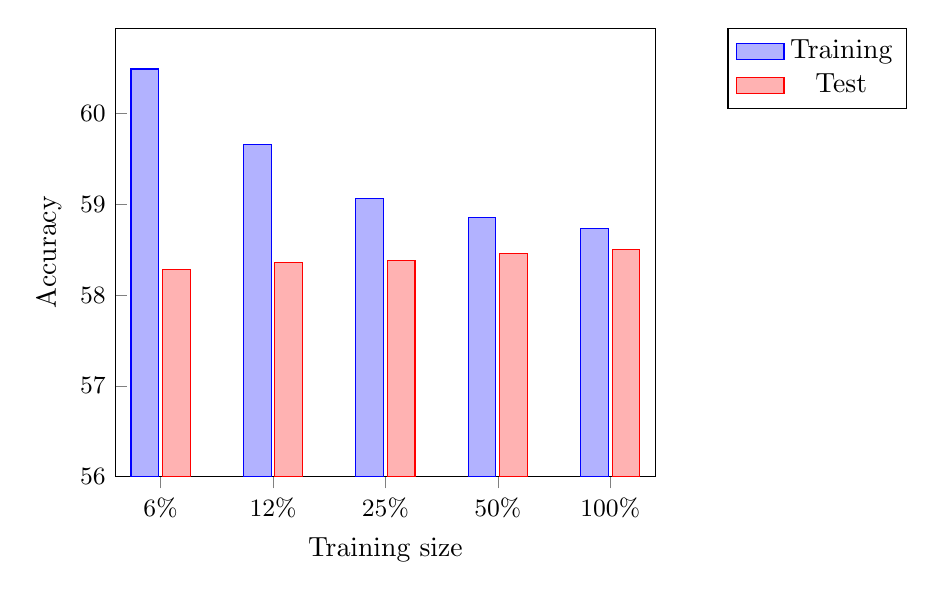
\begin{tikzpicture}
\begin{axis}[
    ybar,
    ylabel = Accuracy,
    xlabel = Training size,
    tick label style={font=\small},
    tickpos=left,
    xticklabels={6\%, 12\%, 25\%, 50\%, 100\%}, 
    xtick={1,2,3,4,5, 6},
    ymin=56,
    legend entries={Training,Test},
    legend style={at={(1.3,1.0)},
        anchor=north,legend columns=1
    },
    legend image code/.code={%
      \draw[#1] (0cm,-0.1cm) rectangle (0.6cm,0.1cm);
    }   
    ]   
    \addplot +[bar shift=-.2cm] coordinates {(1,60.49) (2,59.66) (3,59.06)  (4,58.85)     (5,58.73)  };

    \addplot  +[bar shift=.2cm]coordinates {(1,58.28) (2,58.36) (3,58.38) (4,  58.46) (5,58.50) };

\end{axis}
\end{tikzpicture}
  \caption{Test for representation of features}\label{fig:clusterbigdata}
\end{figure}
The results from \Cref{fig:clusterbigdata} shows that as more data is used to train the model the prediction accuracy on the test set increases the total change from 84529 matches to 134828 matches is $3.86\times10^{-1}\%$

The results also shows the as the size of the training data increases overfitting decreases. The difference in accuracy between the training set and test set moves from $3.79\%$ for $84529$ matches to $3.79\times10^{-1} \%$ for $1348428$ matches. The result shows that the model do not improve a lot as the amount of data increases. The test shows that as the amount of data used for training increases overfitting decreases.      
\subsubsection{Big data improvements}
To test if big data gives an improvement when predicting the outcome of a match, the same features and method where used on an increasing sized data starting from 1000 matches. After the model was made, it was tested on the training data, as a $\frac{2}{3}$-split and finally cross-validation. And as seen on \Cref{fig:bigdata} there will be more information once more tests has been run!

\begin{figure}[!htb]
  \centering
  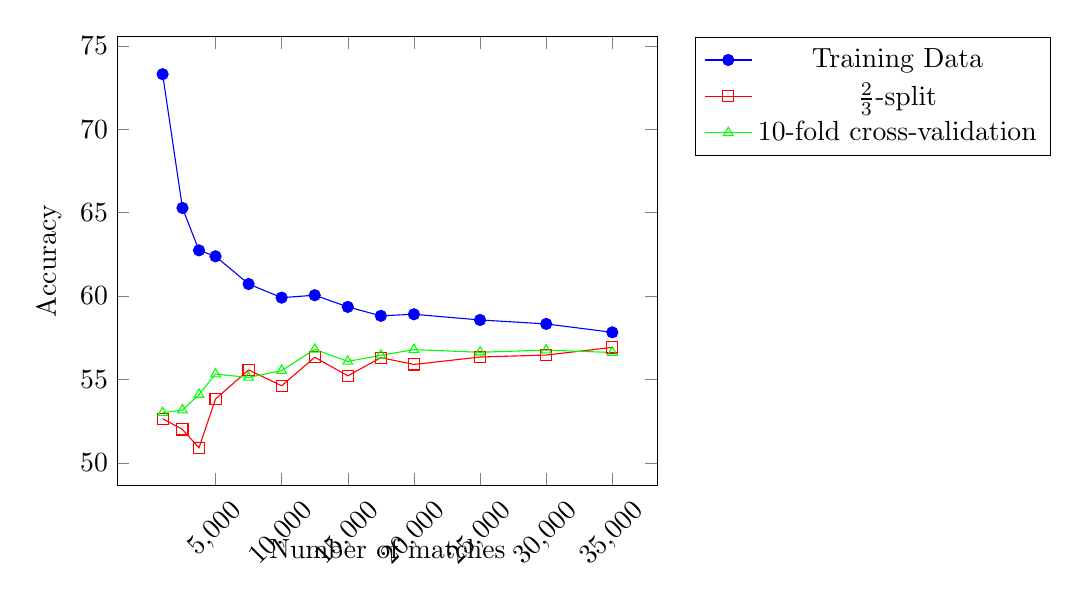
\begin{tikzpicture}[] 
    \begin{axis}[
      xlabel=Number of matches, 
      ylabel=Accuracy,
      xtick={5000,10000,15000,20000,25000,30000,35000},
      xticklabel style={rotate=45,anchor=near xticklabel},
      scaled x ticks=false,
      x label style={at={(axis description cs:0.5,-0.1)},anchor=north},
      legend style={at={(1.4,1.0)},
        anchor=north,legend columns=1},] 
      \addplot[color=blue,mark=*] coordinates {
        (1000, 73.3)    
        (2500,65.28)    
        (3750,62.7367)  
        (5000,62.38)
        (7500,60.72)
        (10000,59.9)
        (12500,60.048)
        (15000,59.3467)
        (17500,58.8114)
        (20000,58.905)
        (25000,58.564)
        (30000,58.3267)
        (35000,57.8229)
      };
      \addplot[color=red,mark=square] coordinates {
        (1000,52.6471)
        (2500,52)
        (3750,50.902)
        (5000,53.8235)
        (7500,55.5686)
        (10000,54.6176)
        (12500,56.3294)
        (15000,55.2157)
        (17500,56.3025)
        (20000,55.8971)
        (25000,56.3412)
        (30000,56.4608)
        (35000,56.916)
      };
      \addplot[color=green,mark=triangle] coordinates {
        (1000,53)
        (2500,53.16)
        (3750,54.0944)
        (5000,55.32)
        (7500,55.12)
        (10000,55.53)
        (12500,56.8)
        (15000,56.08)
        (17500,56.4457)
        (20000,56.785)
        (25000,56.628)
        (30000,56.7567)
        (35000,56.6143)
      };
      \legend{Training Data, $\frac{2}{3}$-split, 10-fold cross-validation}
    \end{axis} 
  \end{tikzpicture}
  \caption{Test for representation of features}\label{fig:bigdata}
\end{figure}

\subsection{Initial testing}\label{sec:initialtest}
In this section several tests will be performed which does not require the cluster. These tests will be run to find the settings the cluster should be run with when the final cluster tests will be performed.

\subsubsection{Best machine learning technique}
First the best machine learning technique needs to be identified. In this test six different methods are tested, which are: naive bayes, hidden naive bayes, logistic regression, neural network, support vector machines(SVM) and adaboost(using decision stump). All the different methods are tested with multiple parameter settings to find the configuration that yields the best result. Note that no parameters are needed for naive bayes and hidden naive bayes. For logistic regression, different L2-regularisation factors have been tested. For SVM, different kernel methods have been tested, namely linear, polynomial, radial, and sigmoid. For Adaboost, different number of iterations have been tested. For neural networks, different number of hidden neurons have been tested, always placed in a single hidden layer.

The feature representation used for this test is binary representation, presented in \Cref{sec:representationoffeatures}, and 35000 matches are used. The data will be split, using $\frac{2}{3}$ for training and $\frac{1}{3}$ for testing. 

The best accuracy we obtained with each of the tested machine learning technique can be seen in \Cref{fig:besttech}. As seen, SVM and Neural networks got the worst accuracy. Naive bayes, adaboost and Hidden naive bayes all have an accuracy close to 56.5\%, but logistic regression has the best accuracy almost hitting 57\%.
The best parameters of each method was found to be:
\begin{itemize}
\item SVM: sigmoid kernel function
\item Adaboost: 200 iterations
\item Logistic regression: L2-regularisation constant = 750
\item Neural Network: $(\text{attributes} + \text{classes}) / 2$ hidden neurons.
\end{itemize}

\begin{figure}[!htb]
  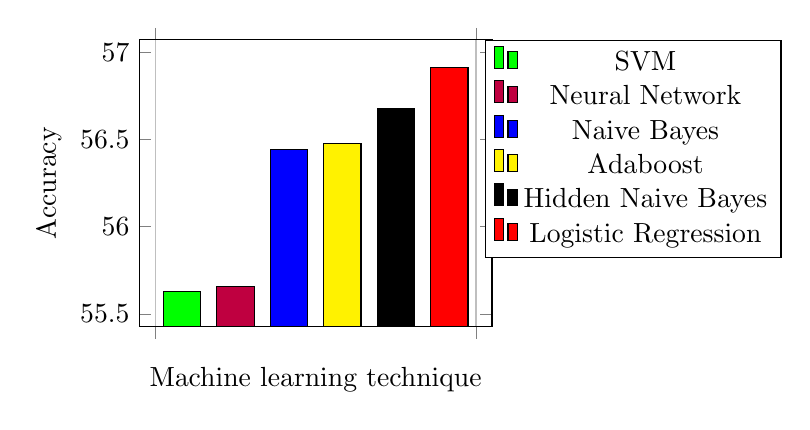
\begin{tikzpicture}
    \begin{axis}[
      %x tick label style={/pgf/number format/1000 sep=},
      xticklabel=\empty,
      ylabel=Accuracy,
      xlabel=Machine learning technique,
      enlargelimits=0.05,
      legend style={at={(1.4,1.0)},
        anchor=north,legend columns=1},
      ybar interval=0.7,
      width=.50\textwidth,
      ymin=55.5, ymax=57,
      reverse legend,
      ]
      \addplot[fill=red] coordinates {(1,56.916) 
        (0,2)
      };
      \addplot[fill=black] coordinates {(1,56.6807) 
        (0,56.6807)
      };
      \addplot[fill=yellow] coordinates {(1,56.479) 
        (0,2)
      };
      \addplot[fill=blue] coordinates {(1,56.4454) 
        (0,56.4454)
      };
      \addplot[fill=purple] coordinates {(1,55.6555) 
        (0,0)
      };
      \addplot[fill=green] coordinates {(1,55.63)
        (0,0)
      };
      \legend{Logistic Regression,Hidden Naive Bayes,Adaboost,Naive Bayes,Neural Network,SVM}
    \end{axis} 
  \end{tikzpicture}
  \caption{Test of best machine learning technique}\label{fig:besttech}
\end{figure}

\subsubsection{Feature symmetry test}
In \Cref{sec:representationoffeatures} we represented four different ways of representing features, to capture a possible symmetry in the choice of champions and the layout of the map. In this section we test each representation by training a classifier using logistic regression using the given representation of features. The test was performed on a test set of 10,000 matches with training sets of up to 50,000 matches. The result, shown in \Cref{fig:feat-rep}, indicates that method 1 and 4 are very close, but as the binary representation is slightly more accurate than the ternary one the majority of the time, we choose to conduct all further tests using the binary representation. 

\begin{figure}[!htb]
  \centering
  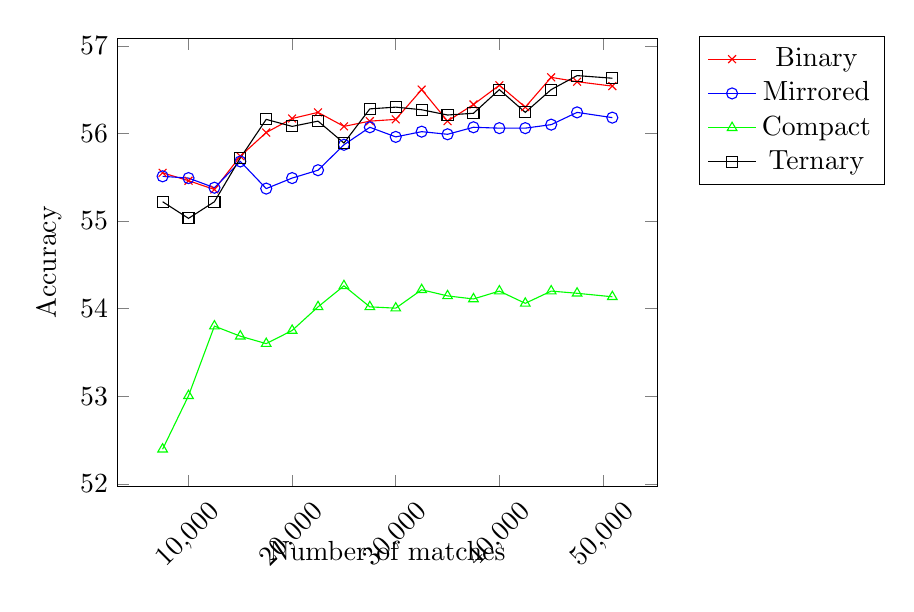
\begin{tikzpicture}[] 
    \begin{axis}[
      xlabel=Number of matches, 
      ylabel=Accuracy,
      xtick={10000,20000,30000,40000,50000},
      xticklabel style={rotate=45,anchor=near xticklabel},
      scaled x ticks=false,
      x label style={at={(axis description cs:0.5,-0.1)},anchor=north},
      legend style={at={(1.25,1.005)},
        anchor=north,legend columns=1},] 
      \addplot[color=red,mark=x] coordinates { 
        (7500, 55.55)
        (10000, 55.46)
        (12500, 55.36)
        (15000, 55.74)
        (17500, 56.01)
        (20000, 56.17)
        (22500, 56.24)
        (25000, 56.08)
        (27500, 56.14)
        (30000, 56.16)
        (32500, 56.50)
        (35000, 56.14)
        (37500, 56.33)
        (40000, 56.55)
        (42500, 56.30)
        (45000, 56.64)
        (47500, 56.59)
        (50901, 56.54)
      };
      \addplot[color=blue,mark=o] coordinates { 
        (7500, 55.51)  
        (10000, 55.49)
        (12500, 55.38)
        (15000, 55.68)
        (17500, 55.37)
        (20000, 55.49)
        (22500, 55.58)
        (25000, 55.87)
        (27500, 56.07)
        (30000, 55.96)
        (32500, 56.02)
        (35000, 55.99)
        (37500, 56.07)
        (40000, 56.06)
        (42500, 56.06)
        (45000, 56.10)
        (47500, 56.24)
        (50901, 56.18)
      };
      \addplot[color=green,mark=triangle] coordinates { 
        (7500, 52.395)  
        (10000, 53.005)
        (12500, 53.80)
        (15000, 53.685)
        (17500, 53.60)
        (20000, 53.75)
        (22500, 54.02)
        (25000, 54.26)
        (27500, 54.02)
        (30000, 54.005)
        (32500, 54.215)
        (35000, 54.145)
        (37500, 54.11)
        (40000, 54.20)
        (42500, 54.06)
        (45000, 54.20)
        (47500, 54.175)
        (50901, 54.135)
      };
      \addplot[color=black,mark=square] coordinates {
        (7500, 55.22)  
        (10000, 55.03)
        (12500, 55.22)
        (15000, 55.72)
        (17500, 56.16)
        (20000, 56.08)
        (22500, 56.14)
        (25000, 55.89)
        (27500, 56.28)
        (30000, 56.30)
        (32500, 56.27)
        (35000, 56.21)
        (37500, 56.23)        
        (40000, 56.50)
        (42500, 56.24)
        (45000, 56.50)
        (47500, 56.66)
        (50901, 56.63)
      };
      \legend{Binary, Mirrored, Compact, Ternary}
    \end{axis} 
  \end{tikzpicture}
  \caption{Test for representation of features}\label{fig:feat-rep}
\end{figure}

\begin{figure}[!htb]
  \centering
  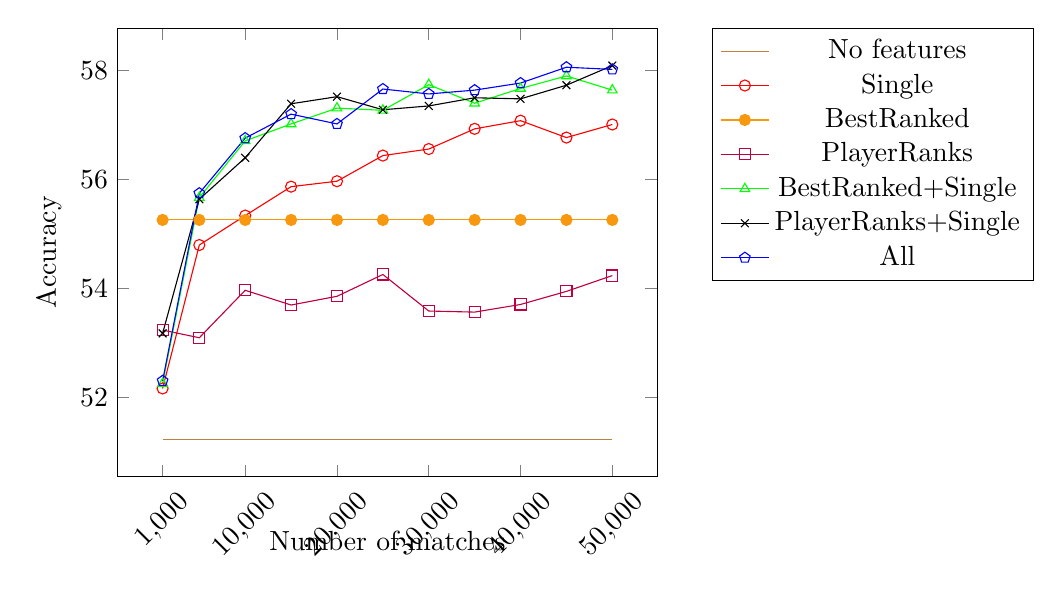
\begin{tikzpicture}[] 
    \begin{axis}[
      xlabel=Number of matches, 
      ylabel=Accuracy,
      xtick={1000,10000,20000,30000,40000,50000},
      xticklabel style={rotate=45,anchor=near xticklabel},
      scaled x ticks=false,
      x label style={at={(axis description cs:0.5,-0.1)},anchor=north},
      legend style={at={(1.4,1.001)},
        anchor=north,legend columns=1},] 
      \addplot[color=brown] coordinates { 
        (1000,51.24)
        (5000,51.24)
        (10000,51.24)
        (15000,51.24)
        (20000,51.24)
        (25000,51.24)
        (30000,51.24)
        (35000,51.24)
        (40000,51.24)
        (45000,51.24)
        (50000,51.24)
      };
      \addplot[color=red,mark=o] coordinates { 
        (1000,52.17)
        (5000,54.8)
        (10000,55.34)
        (15000,55.87)
        (20000,55.97)
        (25000,56.44)
        (30000,56.56)
        (35000,56.93)
        (40000,57.08)
        (45000,56.77)
        (50000,57.01)
      };
      \addplot[color=YellowOrange,mark=*] coordinates { 
        (1000,55.26)
        (5000,55.26)
        (10000,55.26)
        (15000,55.26)
        (20000,55.26)
        (25000,55.26)
        (30000,55.26)
        (35000,55.26)
        (40000,55.26)
        (45000,55.26)
        (50000,55.26)
      };
      \addplot[color=purple,mark=square] coordinates { 
        (1000,53.24)
        (5000,53.1)
        (10000,53.97)
        (15000,53.7)
        (20000,53.86)
        (25000,54.26)
        (30000,53.59)
        (35000,53.57)
        (40000,53.71)
        (45000,53.95)
        (50000,54.24)
      };
      \addplot[color=green,mark=triangle] coordinates { 
        (1000,52.26)
        (5000,55.67)
        (10000,56.71)
        (15000,57.02)
        (20000,57.31)
        (25000,57.27)
        (30000,57.74)
        (35000,57.4)
        (40000,57.67)
        (45000,57.9)
        (50000,57.64)
      };
      \addplot[color=black,mark=x] coordinates { 
        (1000,53.18)
        (5000,55.64)
        (10000,56.4)
        (15000,57.39)
        (20000,57.52)
        (25000,57.28)
        (30000,57.35)
        (35000,57.5)
        (40000,57.48)
        (45000,57.73)
        (50000,58.09)
      };
      \addplot[color=blue,mark=pentagon] coordinates { 
        (1000,52.31)
        (5000,55.75)
        (10000,56.76)
        (15000,57.2)
        (20000,57.02)
        (25000,57.66)
        (30000,57.57)
        (35000,57.64)
        (40000,57.77)
        (45000,58.06)
        (50000,58.02)
      };
      \legend{No features,Single,BestRanked,PlayerRanks,BestRanked+Single,PlayerRanks+Single,All}
    \end{axis} 
  \end{tikzpicture}
  \caption{Accuracy of features}\label{fig:best-feat}
\end{figure}
\subsection{Cluster tests}\label{sec:clustertest}
In this section we perform a number of tests on a cluster setup. The cluster setup becomes import due to large size of data used for these tests.
We use a 2/3 split on all of our data, yielding 1348428 games for training and 577552 for testing.
\todo{skriv mere}
\subsubsection{Feature tests}\label{sec:feattest}
A number of tests are performed to see if combining different types of features may be beneficial.
Tests are performed using logistic regression using stochastic gradient descent and L2 regularisation with a ridge value of 0.01. 
For each feature test 1348428 games are used for training and 577552 games are used for evaluation. 
The different types of features tested are:
\begin{enumerate}
\item $\phi_\text{SINGLE}$
\item $\phi_\text{PAIR}$
\item $\phi_\text{SINGLE}$, $\phi_\text{PAIR}$
\item $\phi_\text{SINGLE}$, $\phi_\text{PAIR}$, $\phi_\text{COUNTER}$
\item $\phi_\text{SINGLE}$, $\phi_\text{PAIR}$, $\phi_\text{COUNTER}$, $\phi_\text{BEST-RANK}$
\end{enumerate}

\begin{figure}[!htb]
  \centering
  % Graph for feature tests. 
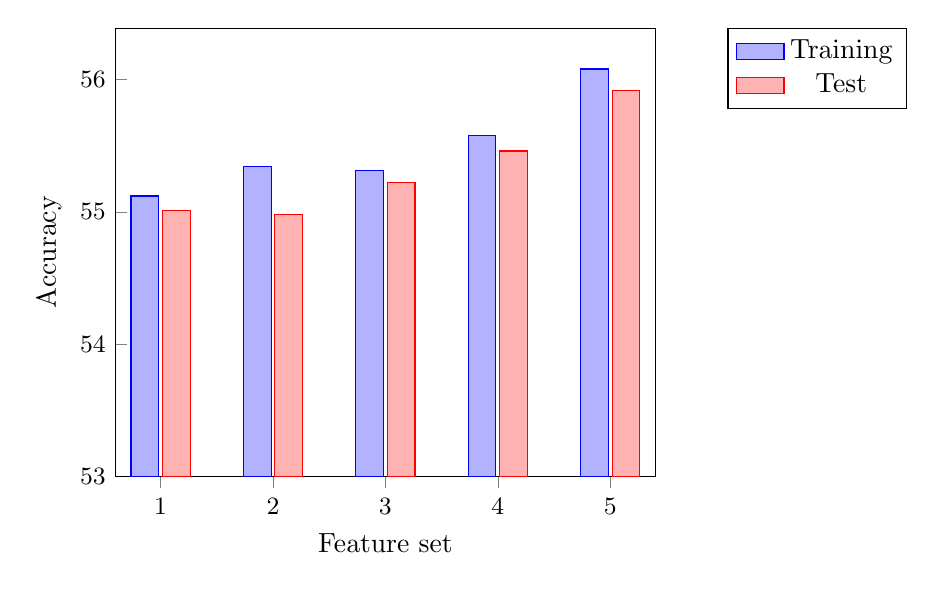
\begin{tikzpicture}
\begin{axis}[
    ybar,
    ylabel = Accuracy,
    xlabel = Feature set,
    tick label style={font=\small},
    tickpos=left,
    xticklabels={1, 2, 3, 4, 5}, 
    xtick={1,2,3,4,5},
    ymin=53,
    legend entries={Training,Test},
    legend style={at={(1.3,1.0)},
        anchor=north,legend columns=1
    },
    legend image code/.code={%
      \draw[#1] (0cm,-0.1cm) rectangle (0.6cm,0.1cm);
    }   
    ]   
    \addplot +[bar shift=-.2cm] coordinates {(1,55.12) (2,55.34) (3,55.31)  (4,55.58)     (5,56.08)};

    \addplot  +[bar shift=.2cm]coordinates {(1,55.01) (2,54.98) (3,55.22) (4,  55.46) (5,55.92)};

\end{axis}
\end{tikzpicture}
   \caption{Accuracy of features}\label{fig:cluster-feat}
\end{figure}

The feature evaluation results from \Cref{fig:cluster-feat} shows two interesting results, by looking at each individual test case we see the we have almost no overfitting. The largest difference is data point 2: (pairs) with a difference of $3.610^{-3}$ percentage points. The results shows some tendency between the complexity of the model and the performance of the classifier. Higher complexity in general yields a better classifier. The best result was achieved using all pre-match features.





\subsection{Knowledge Extraction}\label{sub:knowledge}
In this section we are going to compile an overview of some knowledge which we have extracted from the data. 

While experimenting with various features, we found various weights which seem to be very indicative of the outcome of the match. In this section we will list some of them. It is useful to list these, because they imply a good strategy in the game.

Firstly, one should know that no weights were much higher than others, which would imply the game is relatively balanced! If the opposite was the case, certain strategies would be too good. Which probably would result in a patch that would rebalance the game. Also note that the weights of our model are mostly symmetric around 0, which implies that the game is somewhat symmetric across the two teams. It is also important to realise the weights are based on the matches in our dataset, and the symmetric match might not have been played. 

Note that the sign implies which team the feature is good for. Since we are predicting if blue team wins, negative features are bad for the blue team. The most notable counter pair features:
\begin{itemize}
    \item[$-$] Jinx-BLUE-VS-LeeSin-PURPLE 
    \item[$-$] Blitzcrank-BLUE-VS-LeeSin-PURPLE 
    \item[$+$] LeeSin-BLUE-VS-Blitzcrank-PURPLE 
\end{itemize} 
This means that the champion Jinx is bad versus LeeSin, to explain this one can look at their abilities. Jinx dies easily, but deal high damage, while LeeSin can teleport close to enemies and deal high damage. Blitzcrank versus LeeSin and Nidalee, might be bad for Blitzcrank because he can pull enemies close to him and deal damage, but LeeSin can quickly jump away from Blitzcrank.

Single champions 
\begin{itemize}
    \item[$-$] Bard-PURPLE 
    \item[$-$] Sejuani-PURPLE
    \item[$+$] Blitzcrank-BLUE 
    \item[$+$] Azir-PURPLE
\end{itemize}

Most of these features directly correlate to the average winrate of each champion. In this case Bard, Sejuani and Blitzcrank have the highest winrates individually while Azir has the lowest winrate.

We also defined the feature vector \Cref{eq:best-rank}, this is by far the best feature. That is, the team with the highest rank will often be the winner.


\textcolor{red}{ADD MORE WHEN TESTS ARE DONE, MAYBE REMOVE SOME}



\subsubsection{Low accuracy}

We are not able to achieve a higher accuracy and there are two options why this is the case. We have not used thoroughly representing features or the maximally achievable accuracy is close to ours and it is simply not possible to get a better accuracy. There is not much we can do about the first point, but we definitely have tested with a lot of different features. But then, why is it the case that we can not achieve higher accuracy? It is quite clear that the intention of the game maker is to balance the game, such that no champion or combination of champions is too powerful. If one champion becomes too strong it will be changed and reduced in power. If we look at the newest version of the game, the champions which we have selected as strong and weak have had their power changed. It is definitely the case that picking certain champions or even picking a counter to the enemy champion, will make winning the game easier, but skill is also very important.

\todo{need more text here}

%%% Local Variables:
%%% mode: latex
%%% TeX-master: "../main"
%%% End:



\section{Conclusion}

\bibliography{Literature}



% APPENDIX
\newpage
\appendix
\section{Setting up the Cluster}
\label{sec:hadoop}
To set up a cluster with equal settings to ours, all the machines must be running Debian Wheezy 7.0 32-bit (linux) and connected via switch with static ip. In addiction, one machine must be chosen as the master and the following packages must be installed on all machines:
\begin{itemize}
\item openssh 
\item openssh-server 
\item openjdk-7-jre 
\item openjdk-7-jdk 
\end{itemize}
Now create a new user for the cluster setup, this is considered good practice. The \emph{username} must be the same name across all machines.
\lstset{language=bash}
\begin{lstlisting}
  adduser ``username''
\end{lstlisting} %Maybe rethink quotes in the listing
To easier work with the IP's of the machines, set up a file called \emph{hosts}:
\begin{verbatim}
127.0.0.1 localhost

ip node1
ip node2
ip node3
...
\end{verbatim}
Which is saved in the hosts directory: 
\begin{verbatim}
/etc/hosts
\end{verbatim}
Following that, each machine needs ssh configured, where \emph{node-id} is the alias created in the \emph{hosts} file. Run the following commands in the terminal of each master to each slave and from each slave to master:
\begin{lstlisting}
  ssh-keygen
  ssh-copy-id ``username@node-id''
\end{lstlisting}

\subsection{Setting up Hadoop}
All of the following steps must be done on all machines. To set up Hadoop, create a hadoop group, then add the users previously created to that group:
\begin{lstlisting}
  addgroup hadoop
  adduser ``username'' hadoop
\end{lstlisting}
At this point Hadoop 2.6.0 32-bit should be downloaded and installed in the path \textsf{/usr/local/hadoop}. We then change the owner of the hadoop directory so we have the correct access:
\begin{lstlisting}
  chown -R username:username /usr/local/hadoop
\end{lstlisting}
The following will be put in \emph{/home/username/.bashrc} file:
\begin{verbatim}
export JAVA_HOME=/usr/lib/jvm/java-7-openjdk-i386
export HADOOP_INSTALL=/usr/local/hadoop
export PATH=$PATH:$HADOOP_INSTALL/bin
export PATH=$PATH:$HADOOP_INSTALL/sbin
export HADOOP_MAPRED_HOME=$HADOOP_INSTALL
export HADOOP_COMMON_HOME=$HADOOP_INSTALL
export HADOOP_HDFS_HOME=$HADOOP_INSTALL
export YARN_HOME=$HADOOP_INSTALL
\end{verbatim}
In the file \emph{hadoop-env.sh} found in \textsf{/usr/local/hadoop/etc/hadoop/} the line \emph{JAVA\_HOME} should be replaced with \emph{export JAVA\_HOME=/usr/lib/java-7-openjdk-i386}.
In addition the \emph{core-site.xml} which is found in \textsf{/usr/local/hadoop/etc/hadoop/} needs an added property inside the configuration tag: 
\begin{verbatim}
<property>
  <name>fs.defaultFS</name>
  <value>hdfs://MASTER:9000</value>
</property>
\end{verbatim}
\emph{MASTER} needs to be replaced with the hostname for the master node. Another file that needs added properties is \emph{hdfs-site.xml}, which can be found in the folder \textsf{/usr/local/hadoop/etc/hadoop/}:
\begin{verbatim}
<property>
  <name>dfs.namenode.data.dir</name>
  <value>file:/home/username/data/hdfs/namenode</value>
</property>

<property>
  <name>dfs.datanode.data.dir</name>
  <value>file:/home/username/data/hdfs/datanode</value>
</property>
\end{verbatim}
These should also be added in the configuration tag.
The final thing that needs for Hadoop to run is for the master to know the slaves. Create a file called \emph{slaves} in \textsf{/usr/local/hadoop/etc/hadoop/} with all the hostnames of slaves listed separated by newline:
\begin{verbatim}
node1
node2
...
\end{verbatim}

\subsection{Setting up Apache Spark}
All of the following steps must done on all machines. To get Spark 1.2.1 running, download the hadoop 32-bit precompiled version and install it to \textsf{/usr/local/spark} and again run the command to set up the correct rights:
\begin{lstlisting}
  chown -R username:username/usr/local/spark
\end{lstlisting}
The final step for setting up Apache Spark is copying the previous \emph{slaves} file into the folder \textsf{/usr/local/spark/conf/}.

\subsection{Starting the cluster}
To start the cluster the master has to run the following commands:
\begin{lstlisting}
  start-dfs.sh
  cd /usr/local/spark
  ./sbin/start-all.sh
\end{lstlisting}
Now the cluster is ready to use.

\subsection{Adding files}
To add files to the file system use the following script:
\begin{lstlisting}
  string = $(hdfs dfs -ls hdfs://node1:9000/)
  for file in "file path"*
  do
  name = $(file##*/)

  if [[$string == *$name* ]]
  then
    echo 'file exists'
  else
    hdfs dfs -copyFromLocal $file hdfs://node1:9000/$name
    echo 'adding new file'
  fi 

  done
\end{lstlisting}
This will add all the files, that does not already exist, from the given folder to the hdfs file system.


%%% Local Variables:
%%% mode: latex
%%% TeX-master: "../main"
%%% End:

%\begin{frame}{Finding the Best Model}

% run on a single machine
Tested Classifiers

\begin{itemize}
\item Naive Bayes 
\item Logistic Regression
\item Neural Network
\item Support Vector Machine
\item Adaboost
\item Hoeffding tree
\item Decision Stump
\end{itemize}
%\vspace{20cm}
\end{frame}

\begin{frame}{Finding the Best Model}
\begin{itemize}
\item Data \begin{itemize}
		\item 2/3 Training
		\item 1/3 Testing
           \end{itemize}
\item Parameters? 

\end{itemize}

\end{frame}

\begin{frame}{Finding the Best Model}

\begin{figure}[!htb]
\centering
  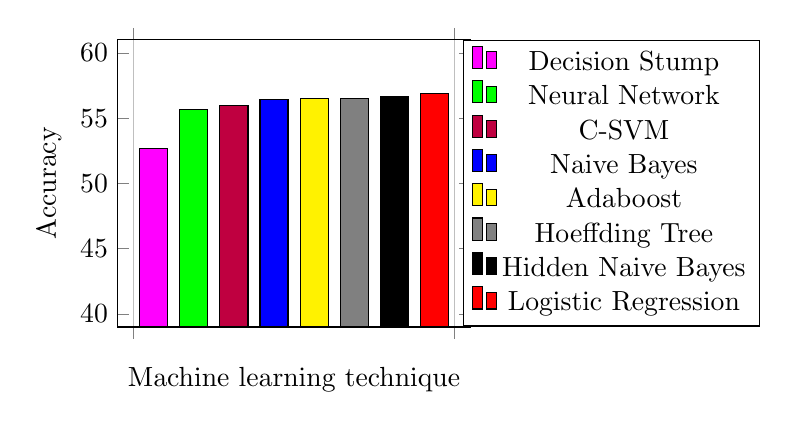
\begin{tikzpicture}
    \begin{axis}[
      %x tick label style={/pgf/number format/1000 sep=},
      xticklabel=\empty,
      ylabel=Accuracy,
      xlabel=Machine learning technique,
      enlargelimits=0.05,
      legend style={at={(1.4,1.0)},
        anchor=north,legend columns=1},
      ybar interval=0.7,
      width=.50\textwidth,
      ymin=40, ymax=60,
      reverse legend,
      ]
      \addplot[fill=red] coordinates {(1,56.916) 
        (0,2)
      };
      \addplot[fill=black] coordinates {(1,56.6807) 
        (0,56.6807)
      };

\addplot[fill=gray] coordinates {(1,56.48)
        (0,0)
      };      
            
      \addplot[fill=yellow] coordinates {(1,56.479) 
        (0,2)
      };
      \addplot[fill=blue] coordinates {(1,56.4454) 
        (0,56.4454)
      };
      \addplot[fill=purple] coordinates {(1,55.98)
        (0,0)
      };
      \addplot[fill=green] coordinates {(1,55.6555) 
        (0,0)
      };      
      \addplot[fill=Fuchsia] coordinates {(1,52.64)
        (0,0)
      };
      \legend{Logistic Regression,Hidden Naive Bayes,Hoeffding Tree,Adaboost,Naive Bayes,C-SVM,Neural Network, Decision Stump}
    \end{axis} 
  \end{tikzpicture}
%  \caption{ue}\label{fig:besttech}
\end{figure}

\end{frame}

\begin{frame}{Logistic Regression}

\[ L_D(\textbf{w}) = \sum_{n=1}^N (y_n-\hat{y}_n)^2 = \sum_{n=1}^N \left(y_n - \sum_{i=0}^M w_i \phi_i(x_n)\right)^{2} \] 

\end{frame}

\begin{frame}{Logistic Regression}

\[ \hat{y} = \sigma(h_w(x)) = \frac{1}{1+e^{-h_w(x)}} \]

\[E_w(y,h_w(x)) = \begin{cases}
	-ln(\sigma(h_w(x))) &\text{if y = 1}\\	
	-ln(1-\sigma(h_w(x))) &\text{if y = 0}
\end{cases}\]

\end{frame}

\begin{frame}{Regularisation}

\[ L(\mathbf{w})
  = L_D(\mathbf{w}) + L_w 
  = \sum_{n=1}^N E_w(y_n, h_w(x_n)) + \frac{\lambda}{2} \sum_{m=1}^{M} {w_m}^2 \] 

\end{frame}

\begin{frame}{Stochastic Gradient Descent}

\[ w_j^{(i)} = w_j^{(i-1)} - \eta \frac{\partial E_{w^{(i-1)}}(y_n, h_{w^{(i-1)}}(x_n))}{\partial w_j^{(i-1)}} \]

\end{frame}


\begin{frame}{Simulated Annealing}

$$\eta_i = \frac{1}{(1+i)^\alpha}$$


With an $\alpha$ chosen in the interval $(0.5,1]$. 

\end{frame}


%\begin{frame}
%\end{frame}



%\section{Data and Feature Setup}\label{sec:features}
In \Cref{sec:matchdata} we investigate the match data made available by the Riot's API, which covers almost any detail of a match.
\Cref{sec:choosingfeatures} identifies a number of features that can be extracted from match data, which we think are most important when it comes to prediction of the winning team. The choice is based on our intuition as more or less experienced LoL players. The size of each type of features domain is calculated in \Cref{sec:featuresparsity}, as well as the sparsity with regards to how many features that appear in each match.
In \Cref{sec:representationoffeatures}, a possible feature symmetry issue is investigated which raises a number of concerns and suggestions for solutions as to how the extracted features should be represented. 


\subsection{League of Legends Match Information}\label{sec:matchdata}
Riot records large amounts of information about played matches and players~\cite{matchinfo}. Much, if not all, of this data is publicly available through their online API. In this paper the focus will be on the match data only, and more particularly the data that can be extracted before a match starts. The only exception is information about which team that won each match. Since we want to predict who wins, we need that data to train and evaluate a classifier.
We have chosen to extract the following data from each match:
\begin{itemize}
\item Winning team
\item Champions on each of the two teams
\item The rank of all players
\item Game mode
\item Queue type
\end{itemize}
And the following data from each player:
\begin{itemize}
\item Lane occupied 
\item Runes 
\item Masteries 
\item Summoner spells 
\end{itemize}
All the extracted information has be chosen because we think it might be useful for estimating how good a particular team is against another team. \todo{kommetar: dårlig begrundelse}
The champions on each of the two teams have been included because some champions may be better than others.
The rank of players are considered because the rank system in LoL aims to assign better players a greater rank. Intuitively, a team of high ranked players must be better than a team of low ranked players.
The lane played by each player may be useful, because players often stick to one particular lane for the first half a match.
Note that the lanes of the opponent team is not known before the game starts, but we have still chosen to include it, because it very often can determined based on the picked champions. Knowing the lane of the players means knowing the ranks and champion of the players that most often fights against each other.
Both the masteries, runes. and summoner spells are worth knowing, because each of them add or improve some property of a champion. 
%The summoner spells are also worth considering because they adds additional properties to a champion.
Different game modes imply different play styles. By only considering the 5 versus 5 game mode, we hope to achieve better predictions.
The queue type of the match lets us know if the LoL match making system has formed the two teams, or the players have formed the two teams themselves.
Teams formed on their own may be better, because the players in self formed teams often know each other better and more often use voice communication tools.
Finally the matches patch version is used to make sure that we only use matches from the same patches. Different patches may change aspects of the game, e.g.\ the strength of particular champions, and without accounting for different patches, the trained classifier accuracy may decrease.  

The data set we use use consists of matches played from $23^{\text{rd}}$ of March 2015 to $27^{\text{th}}$ of March 2015. It includes match details for matches played across the world. When filtering the games to include only 5 versus 5 game modes, we are left with 1925980 matches. The patch version of all matches used is $5.6$.


%%% Local Variables:
%%% mode: latex
%%% TeX-master: "../main"
%%% End:


\end{document}

%%% Local Variables:
%%% mode: latex
%%% TeX-master: t
%%% End:
